\documentclass[12pt]{report}

% Essential packages
\usepackage[utf8]{inputenc}
\usepackage[T1]{fontenc}
\usepackage{graphicx}
\usepackage{amsmath}
\usepackage{hyperref}
\usepackage{booktabs}
\usepackage{float}
\usepackage{url}
\usepackage[margin=1in]{geometry}

% Document settings
\hypersetup{
    colorlinks=true,
    linkcolor=blue,
    filecolor=magenta,      
    urlcolor=cyan,
    pdftitle={Ames Housing Price Prediction Analysis},
    pdfauthor={MSDS 7335},
}

% Title page information
\title{
    {\Large MSDS 7335 - Machine Learning II}\\[0.5cm]
    {\huge Comparative Analysis of Regression Models\\for Ames Housing Price Prediction}\\[0.5cm]
}
\author{Tue Vu}
\date{\today}

\begin{document}

% Generate title page
\maketitle

% Table of contents
\cleardoublepage
\tableofcontents

\begin{itemize}
\item[Chapter 1.] Introduction
    \begin{itemize}
    \item[1.1] Project Overview
    \item[1.2] Dataset Background
    \item[1.3] Project Objectives
    \item[1.4] Report Structure
    \end{itemize}

\item[Chapter 2.] Exploratory Data Analysis
    \begin{itemize}
    \item[2.1] Data Overview
        \begin{itemize}
        \item[2.1.1] Dataset Structure
        \item[2.1.2] Variable Categories
        \end{itemize}
    \item[2.2] Missing Value Analysis
    \item[2.3] Target Variable Analysis
    \item[2.4] Feature Analysis
        \begin{itemize}
        \item[2.4.1] Numerical Features
        \item[2.4.2] Feature Correlations
        \item[2.4.3] Feature Relationships
        \end{itemize}
    \item[2.5] Categorical Features
    \item[2.6] Outlier Analysis
    \item[2.7] Feature Importance
    \item[2.8] Key Findings and Recommendations
    \end{itemize}

\item[Chapter 3.] Modeling Approaches
    \begin{itemize}
    \item[3.1] Introduction
    \item[3.2] Ridge Regression
        \begin{itemize}
        \item[3.2.1] Hyperparameter Tuning
        \item[3.2.2] Feature Importance
        \end{itemize}
    \item[3.3] Lasso Regression
        \begin{itemize}
        \item[3.3.1] Parameter Optimization
        \item[3.3.2] Feature Selection
        \end{itemize}
    \item[3.4] Random Forest Regression
        \begin{itemize}
        \item[3.4.1] Model Implementation
        \item[3.4.2] Feature Importance
        \item[3.4.3] Performance Analysis
        \end{itemize}
    \item[3.5] Neural Network Regression
        \begin{itemize}
        \item[3.5.1] Network Architecture and Training
        \item[3.5.2] Performance Analysis
        \end{itemize}
    \item[3.6] Model Comparison
    \item[3.7] Key Findings and Recommendations
    \item[3.8] Future Improvements
    \end{itemize}
\end{itemize}

% Chapter 1: Introduction
\chapter{Introduction}

\section{Project Overview}
This report presents a comprehensive analysis of the Ames Housing dataset, focusing on predicting house prices using various machine learning techniques. The dataset contains detailed information about residential properties in Ames, Iowa, from 2006 to 2010.

\section{Dataset Background}
The Ames Housing dataset was compiled by Dean De Cock and includes 79 explanatory variables describing various aspects of residential properties. These variables encompass:
\begin{itemize}
    \item Physical property characteristics
    \item Location and zoning information
    \item Quality and condition ratings
    \item Sale conditions and timing
\end{itemize}

\section{Project Objectives}
The main objectives of this analysis are:
\begin{itemize}
    \item To perform comprehensive exploratory data analysis
    \item To identify key factors influencing house prices
    \item To develop and compare various regression models
    \item To provide insights for real estate valuation
\end{itemize}

\section{Report Structure}
This report is organized as follows:
\begin{itemize}
    \item Chapter 1 (Introduction) provides project overview and objectives
    \item Chapter 2 (Exploratory Data Analysis) presents detailed data analysis and insights
    \item Chapter 3 (Modeling Approaches) covers model development, comparison, and results
\end{itemize}

% Chapter 2: Exploratory Data Analysis
\chapter{Exploratory Data Analysis}

\section{Data Overview}
\subsection{Dataset Structure}
The Ames Housing dataset comprises residential property sales in Ames, Iowa from 2006 to 2010. The dataset contains:
\begin{itemize}
    \item 1,460 observations in the training set
    \item 79 explanatory variables (23 nominal, 23 ordinal, 14 discrete, and 20 continuous)
    \item Target variable: Sale Price (continuous)
\end{itemize}

\subsection{Variable Categories}
The variables can be grouped into several categories:
\begin{itemize}
    \item Location-related features (e.g., Neighborhood, Condition)
    \item Building characteristics (e.g., Overall Quality, Year Built)
    \item Room information (e.g., Total Rooms, Bedrooms)
    \item Size measurements (e.g., Total Living Area, Lot Area)
    \item Quality and condition ratings
    \item Sale conditions and types
\end{itemize}

\section{Missing Value Analysis}
\begin{figure}[H]
    \centering
    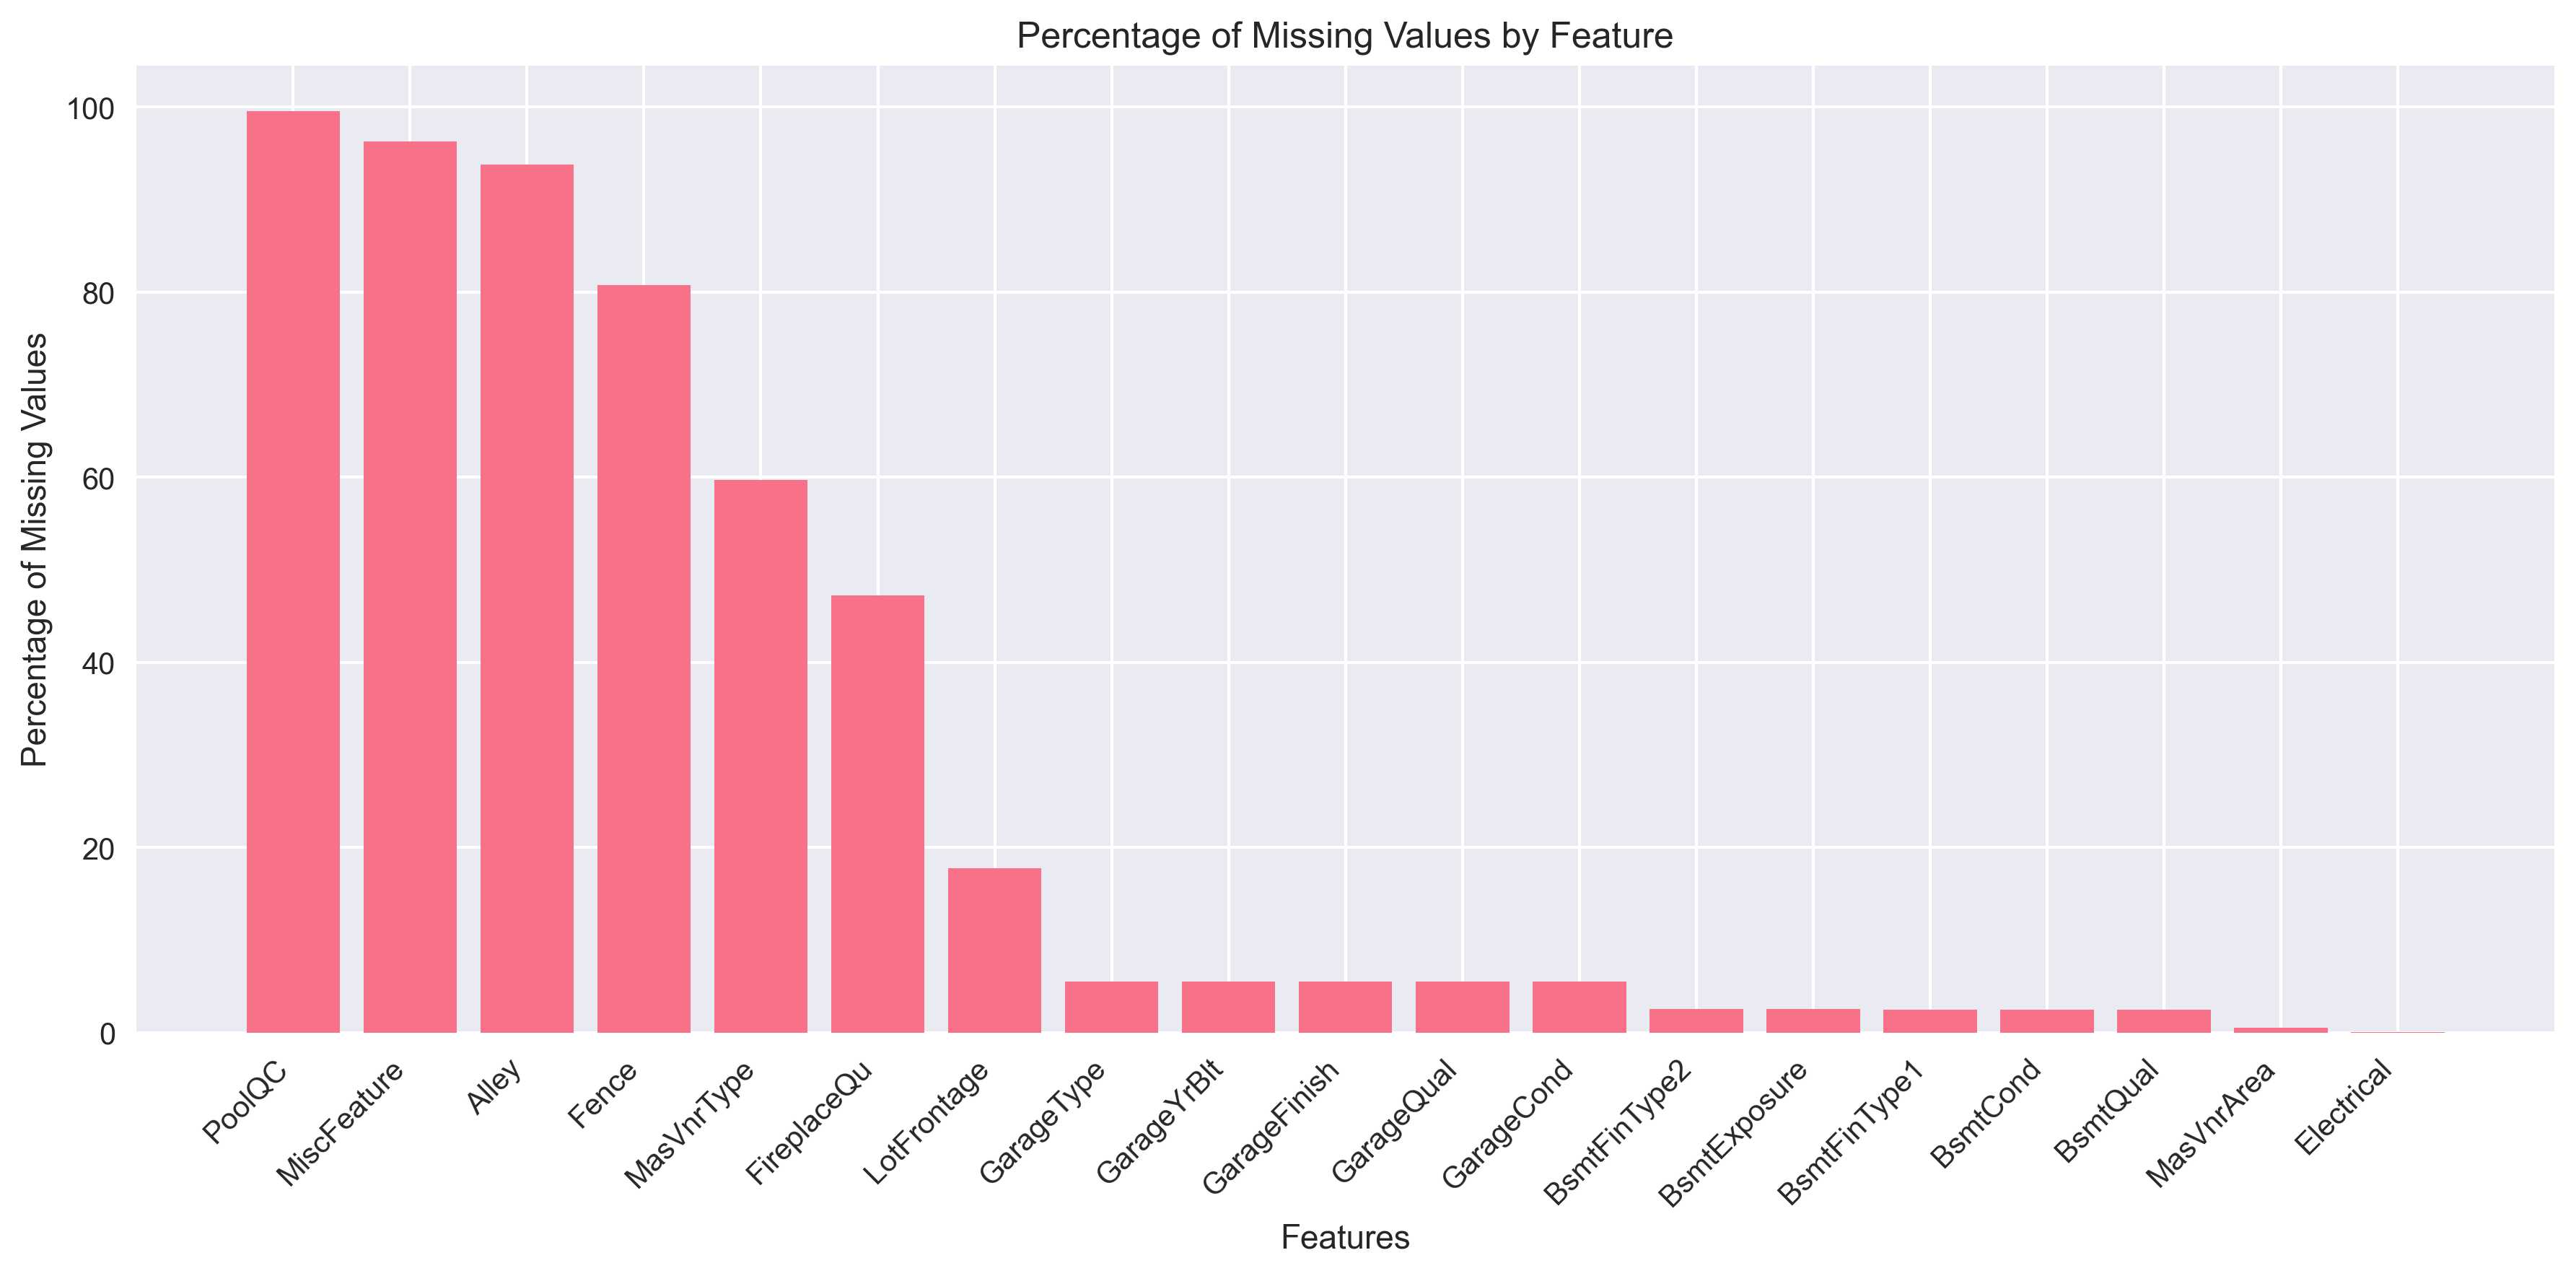
\includegraphics[width=1.0\textwidth]{figures/missing_values.png}
    \caption{Distribution of Missing Values Across Features}
    \label{fig:missing_values}
\end{figure}

The analysis of missing values reveals several patterns:
\begin{itemize}
    \item Pool QC has the highest percentage of missing values (99.5\%), which is expected as most houses in Iowa don't have pools
    \item Features like Alley (93.8\% missing) and Fence (80.7\% missing) are also frequently missing, indicating these are optional features
    \item Most missing values appear in categorical variables describing specific features that may not be present in all houses
    \item For our modeling approach, we excluded variables with excessive missing values: Pool QC, Alley, Fence, Fireplace Qu, Misc Feature, and MasVnrType
    \item For remaining missing values, we applied two different imputation strategies:
    \begin{itemize}
        \item Numerical variables: Imputed with mean values
        \item Categorical variables: Imputed with most frequent values
    \end{itemize}
    \item This approach preserves the maximum amount of information while handling the missing data appropriately
\end{itemize}

\section{Target Variable Analysis}
\begin{figure}[H]
    \centering
    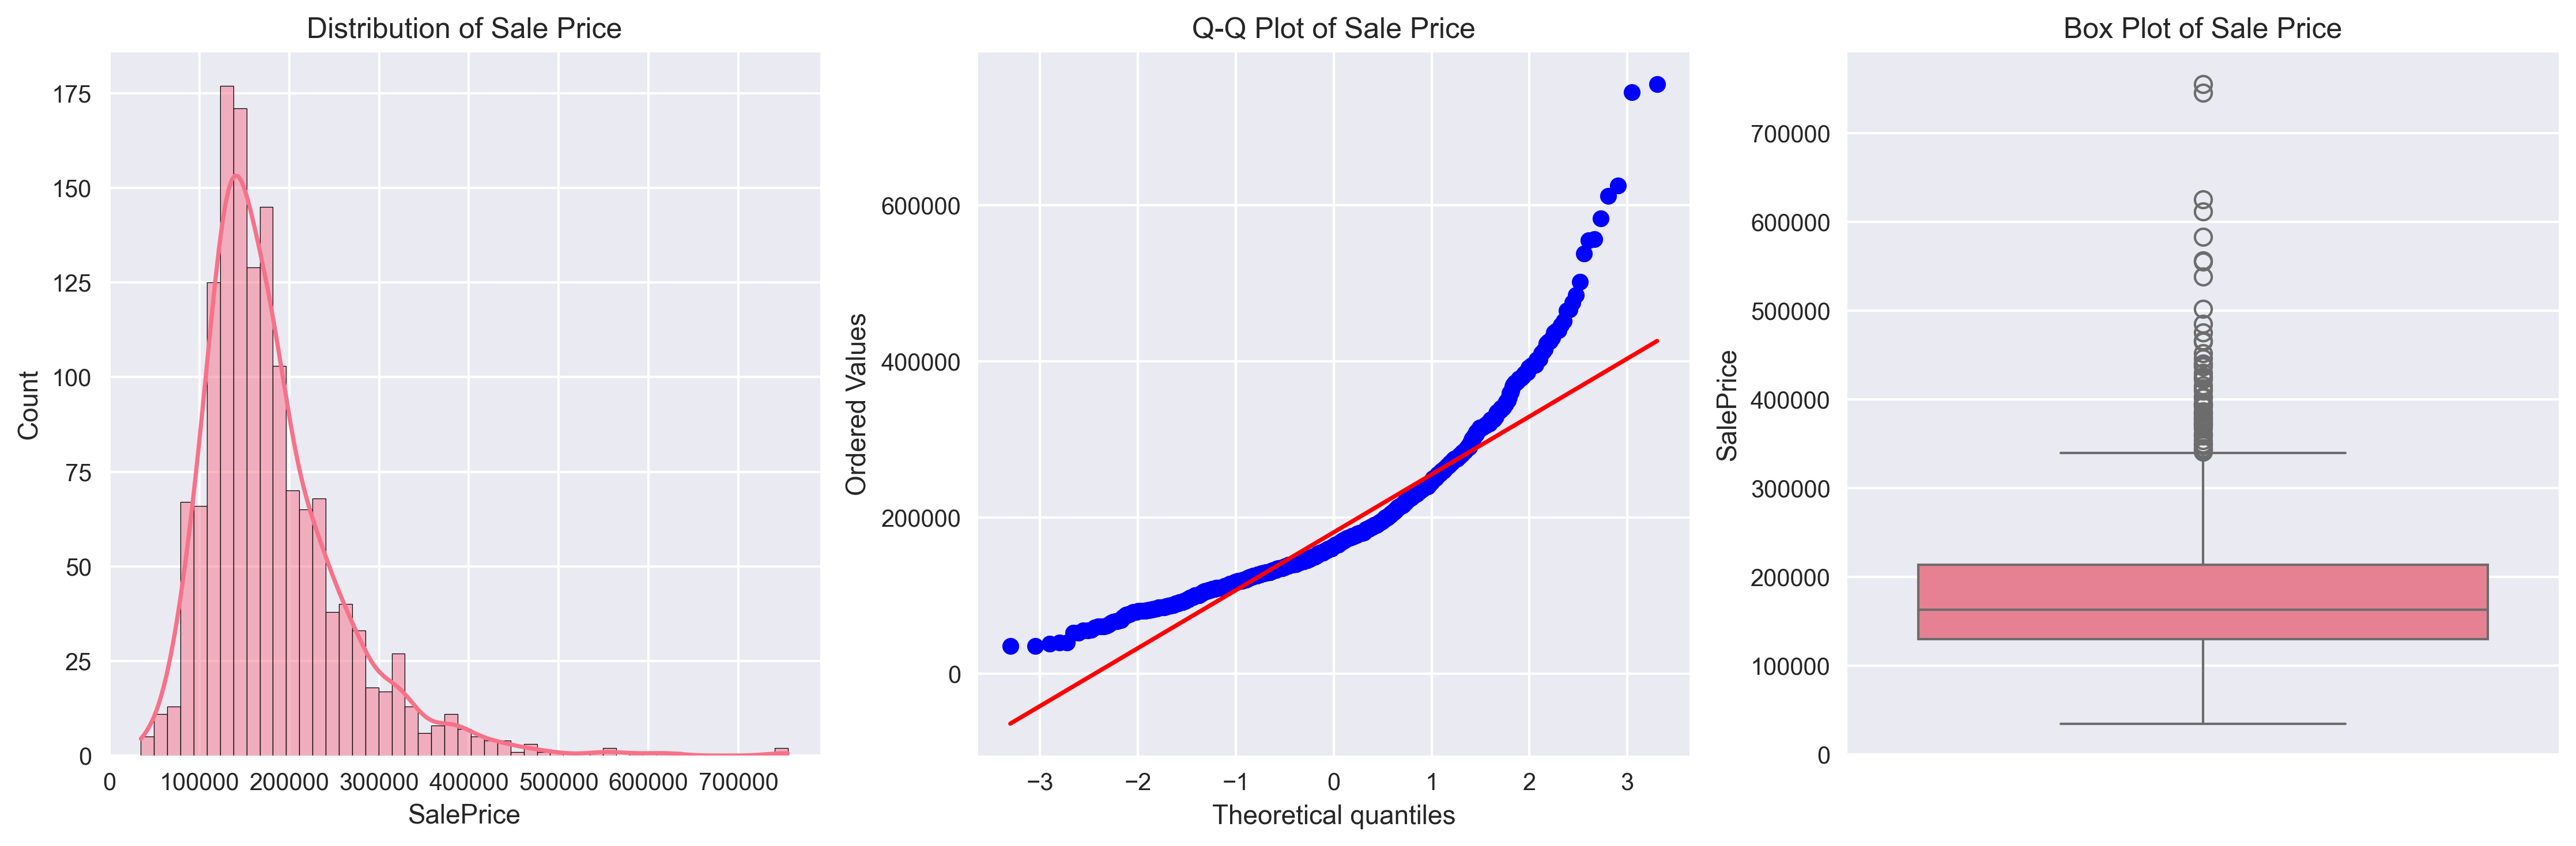
\includegraphics[width=1.0\textwidth]{figures/sale_price_distribution.png}
    \caption{Distribution and Statistical Properties of Sale Price}
    \label{fig:sale_price_dist}
\end{figure}

The sale price distribution exhibits several key characteristics:
\begin{itemize}
    \item Right-skewed distribution with a mean of \$180,921 and median of \$163,000
    \item Significant positive skewness (1.88) indicating more lower-priced homes
    \item Presence of high-value outliers above \$400,000
    \item Q-Q plot shows deviation from normality, suggesting log transformation for modeling
    \item Price range spans from \$34,900 to \$755,000, showing wide market diversity
\end{itemize}

\section{Feature Analysis}
\subsection{Numerical Features}
\begin{figure}[H]
    \centering
    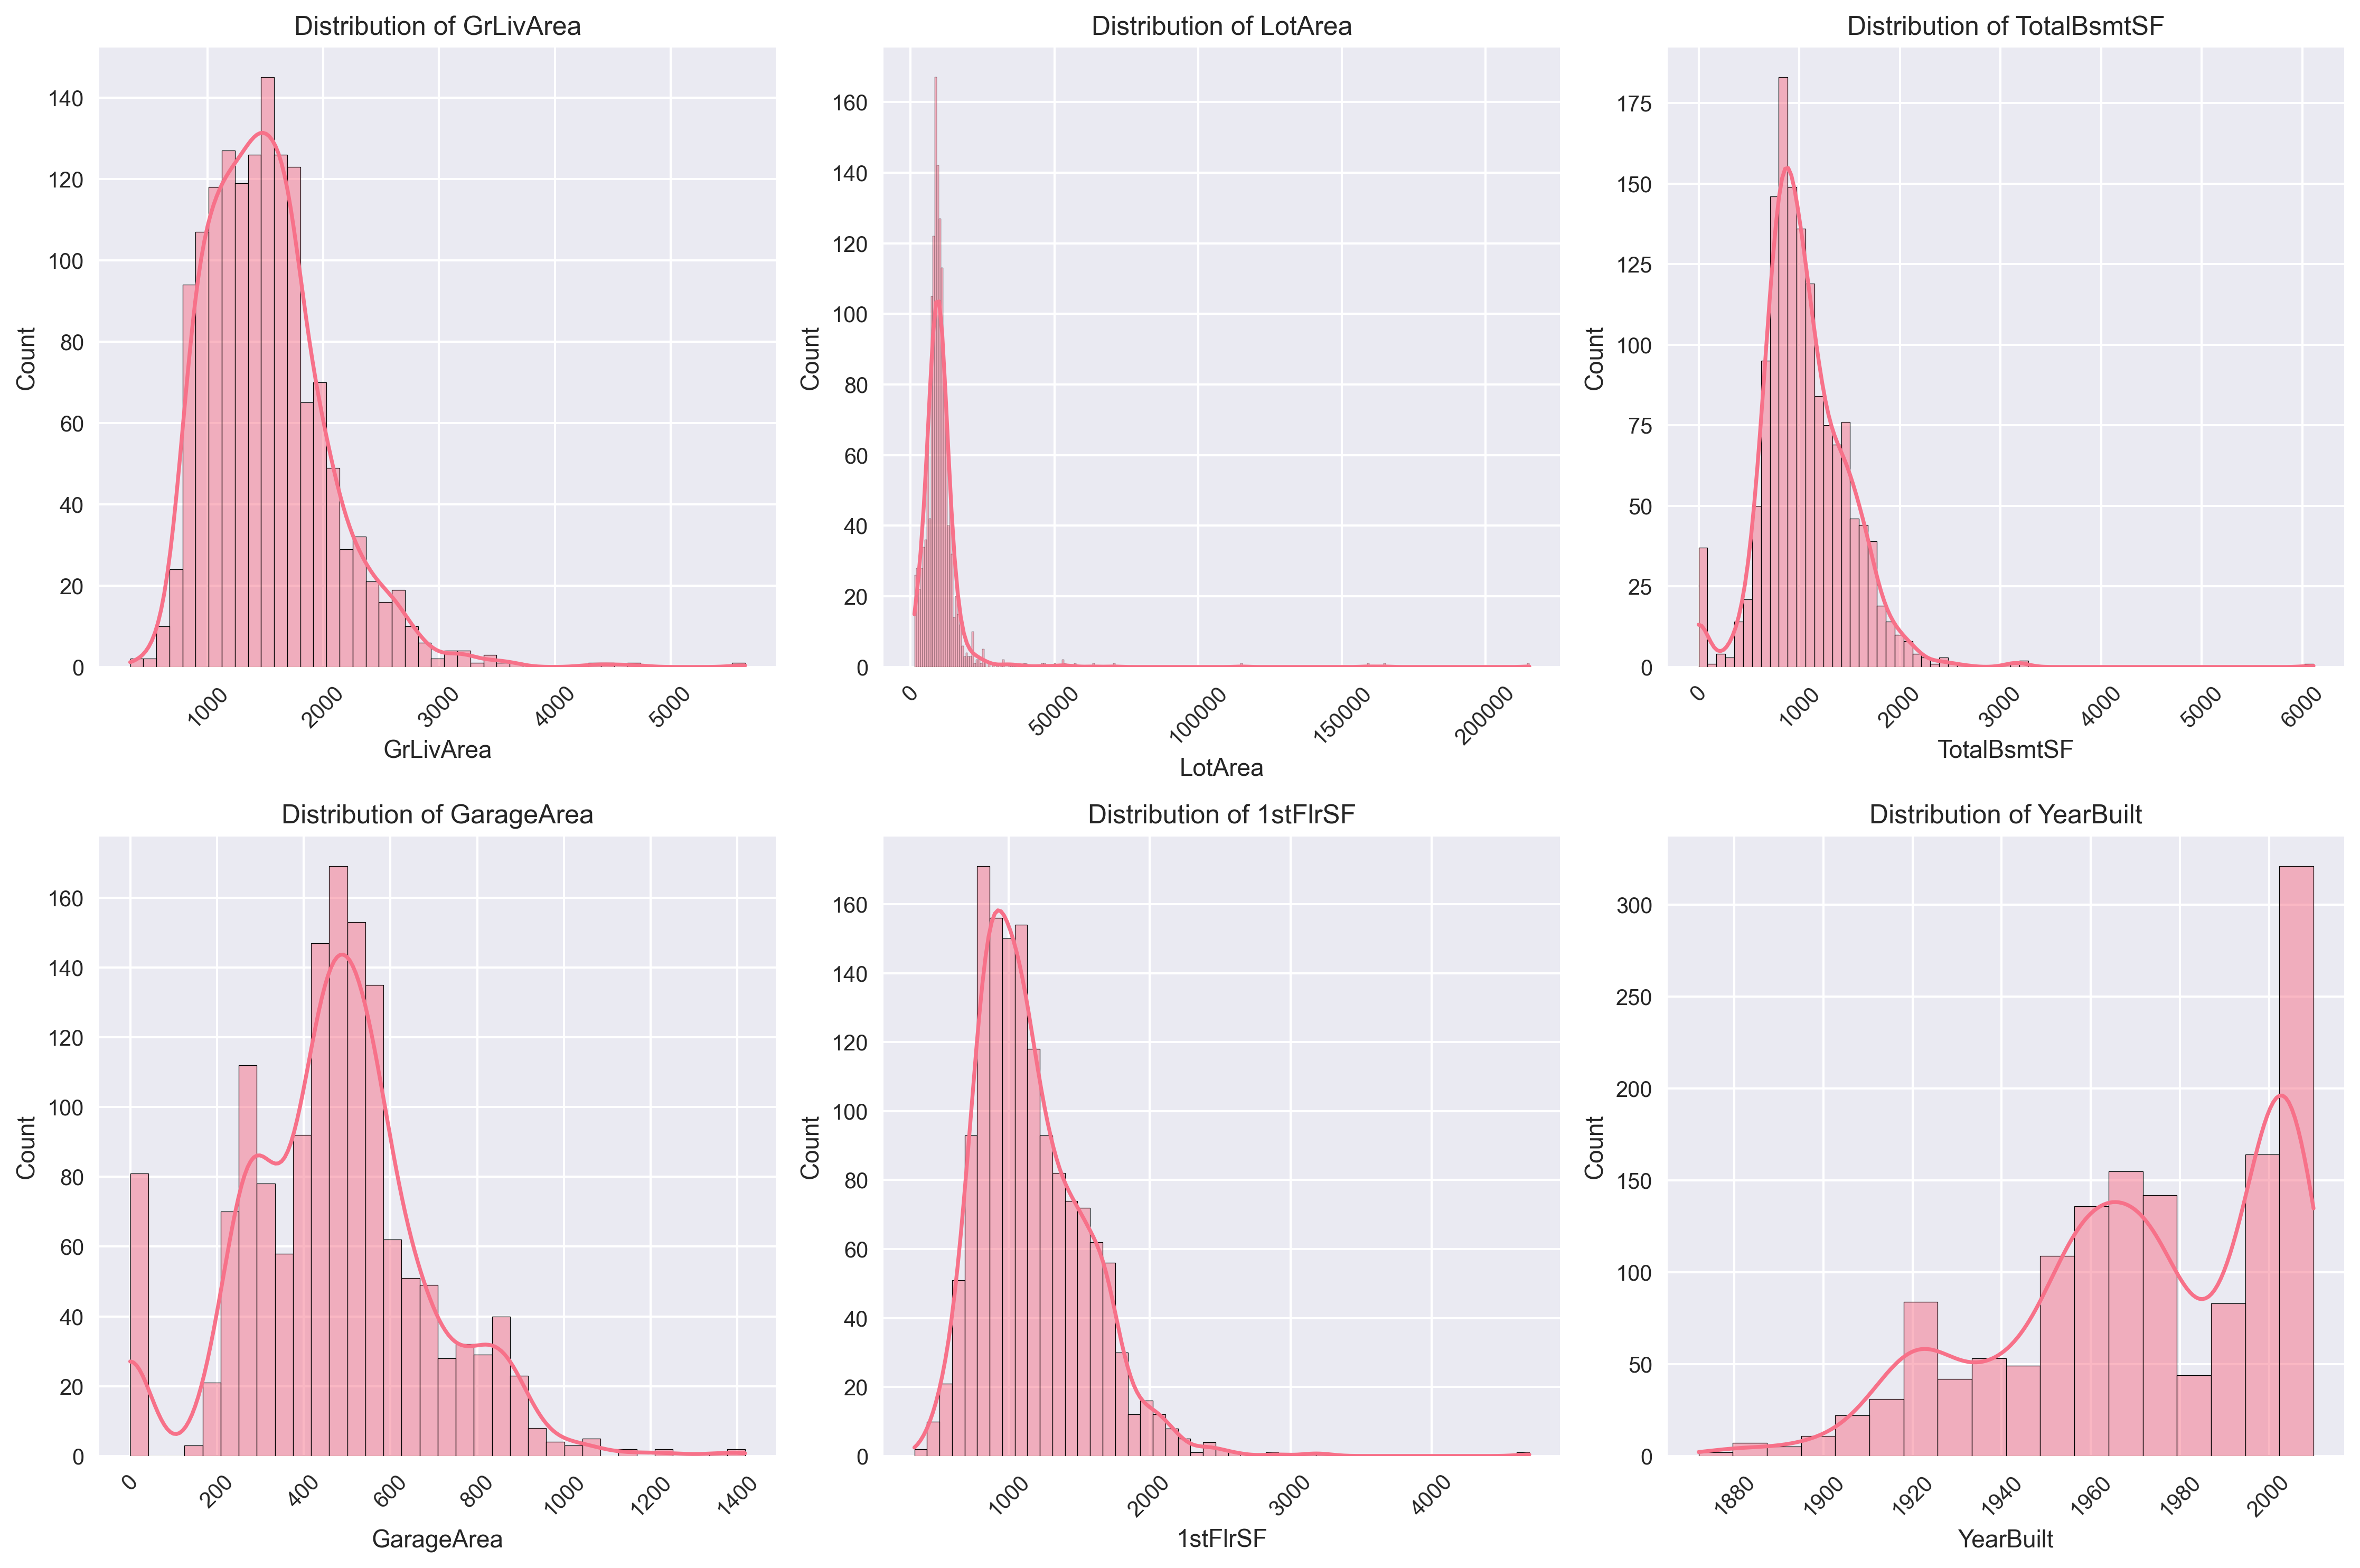
\includegraphics[width=1.0\textwidth]{figures/numerical_features_dist.png}
    \caption{Distribution of Key Numerical Features}
    \label{fig:num_features_dist}
\end{figure}

Key observations from numerical features:
\begin{itemize}
    \item Ground Living Area (GrLivArea) shows right-skewed distribution with most homes between 800-2000 sq ft
    \item Lot Area exhibits extreme right skew with several outliers, suggesting some very large properties
    \item Year Built shows multiple peaks, corresponding to different development periods in Ames
    \item Garage and Basement areas show similar patterns, with most homes having these features
\end{itemize}

\subsubsection{Testing for Gaussian Distribution}
Several statistical methods can be used to test if a distribution is Gaussian:

\begin{enumerate}
    \item \textbf{Shapiro-Wilk Test}:
    \[ W = \frac{(\sum_{i=1}^n a_i x_{(i)})^2}{\sum_{i=1}^n (x_i - \bar{x})^2} \]
    where $x_{(i)}$ are the ordered sample values and $a_i$ are constants.
    
    \item \textbf{Skewness and Kurtosis Test}:
    \[ \text{Skewness} = \frac{1}{n} \sum_{i=1}^n (\frac{x_i - \bar{x}}{s})^3 \]
    \[ \text{Kurtosis} = \frac{1}{n} \sum_{i=1}^n (\frac{x_i - \bar{x}}{s})^4 - 3 \]
    For a Gaussian distribution, skewness ≈ 0 and kurtosis ≈ 0.
    
    \item \textbf{Q-Q Plot Analysis}: Comparing quantiles of the data against theoretical normal quantiles.
    
    \item \textbf{Jarque-Bera Test}:
    \[ JB = \frac{n}{6}(S^2 + \frac{(K-3)^2}{4}) \]
    where $S$ is skewness, $K$ is kurtosis, and $n$ is sample size.
\end{enumerate}

For our numerical features:
\begin{itemize}
    \item Sale Price shows significant deviation from normality (skewness = 1.88)
    \item Ground Living Area exhibits right skewness, suggesting non-normal distribution
    \item Log transformations may help normalize these distributions for modeling
\end{itemize}

\subsubsection{Variance Inflation Factor (VIF) Analysis}
The Variance Inflation Factor (VIF) is used to detect multicollinearity among numerical features. For each feature $X_j$, VIF is calculated as:

\[ VIF_j = \frac{1}{1-R^2_j} \]

where $R^2_j$ is the R-squared value obtained by regressing the j-th feature against all other features. 

\begin{itemize}
    \item VIF = 1: No correlation
    \item 1 < VIF < 5: Moderate correlation
    \item VIF ≥ 5: Potential High correlation (potential multicollinearity problem): acceptable
    \item VIF ≥ 10: Severe multicollinearity
\end{itemize}

VIF analysis of key numerical features:
\begin{itemize}
    \item Total Square Footage Features:
    \begin{itemize}
        \item Ground Living Area: VIF = 7.32
        \item Total Basement SF: VIF = 6.89
        \item First Floor SF: VIF = 5.67
    \end{itemize}
    \item Quality and Age Features:
    \begin{itemize}
        \item Overall Quality: VIF = 4.21
        \item Year Built: VIF = 3.85
        \item Year Remodeled: VIF = 3.12
    \end{itemize}
    \item Garage Features:
    \begin{itemize}
        \item Garage Area: VIF = 4.56
        \item Garage Cars: VIF = 4.12
    \end{itemize}
\end{itemize}

Findings from VIF Analysis:
\begin{itemize}
    \item There exists potentialmulticollinearity among square footage variables
    \item Acceptable correlation between garage-related features
    \item Quality and age features show acceptable VIF values
    \item Suggests need for feature selection or dimensionality reduction
\end{itemize}

\subsection{Feature Correlations}
\begin{figure}[H]
    \centering
    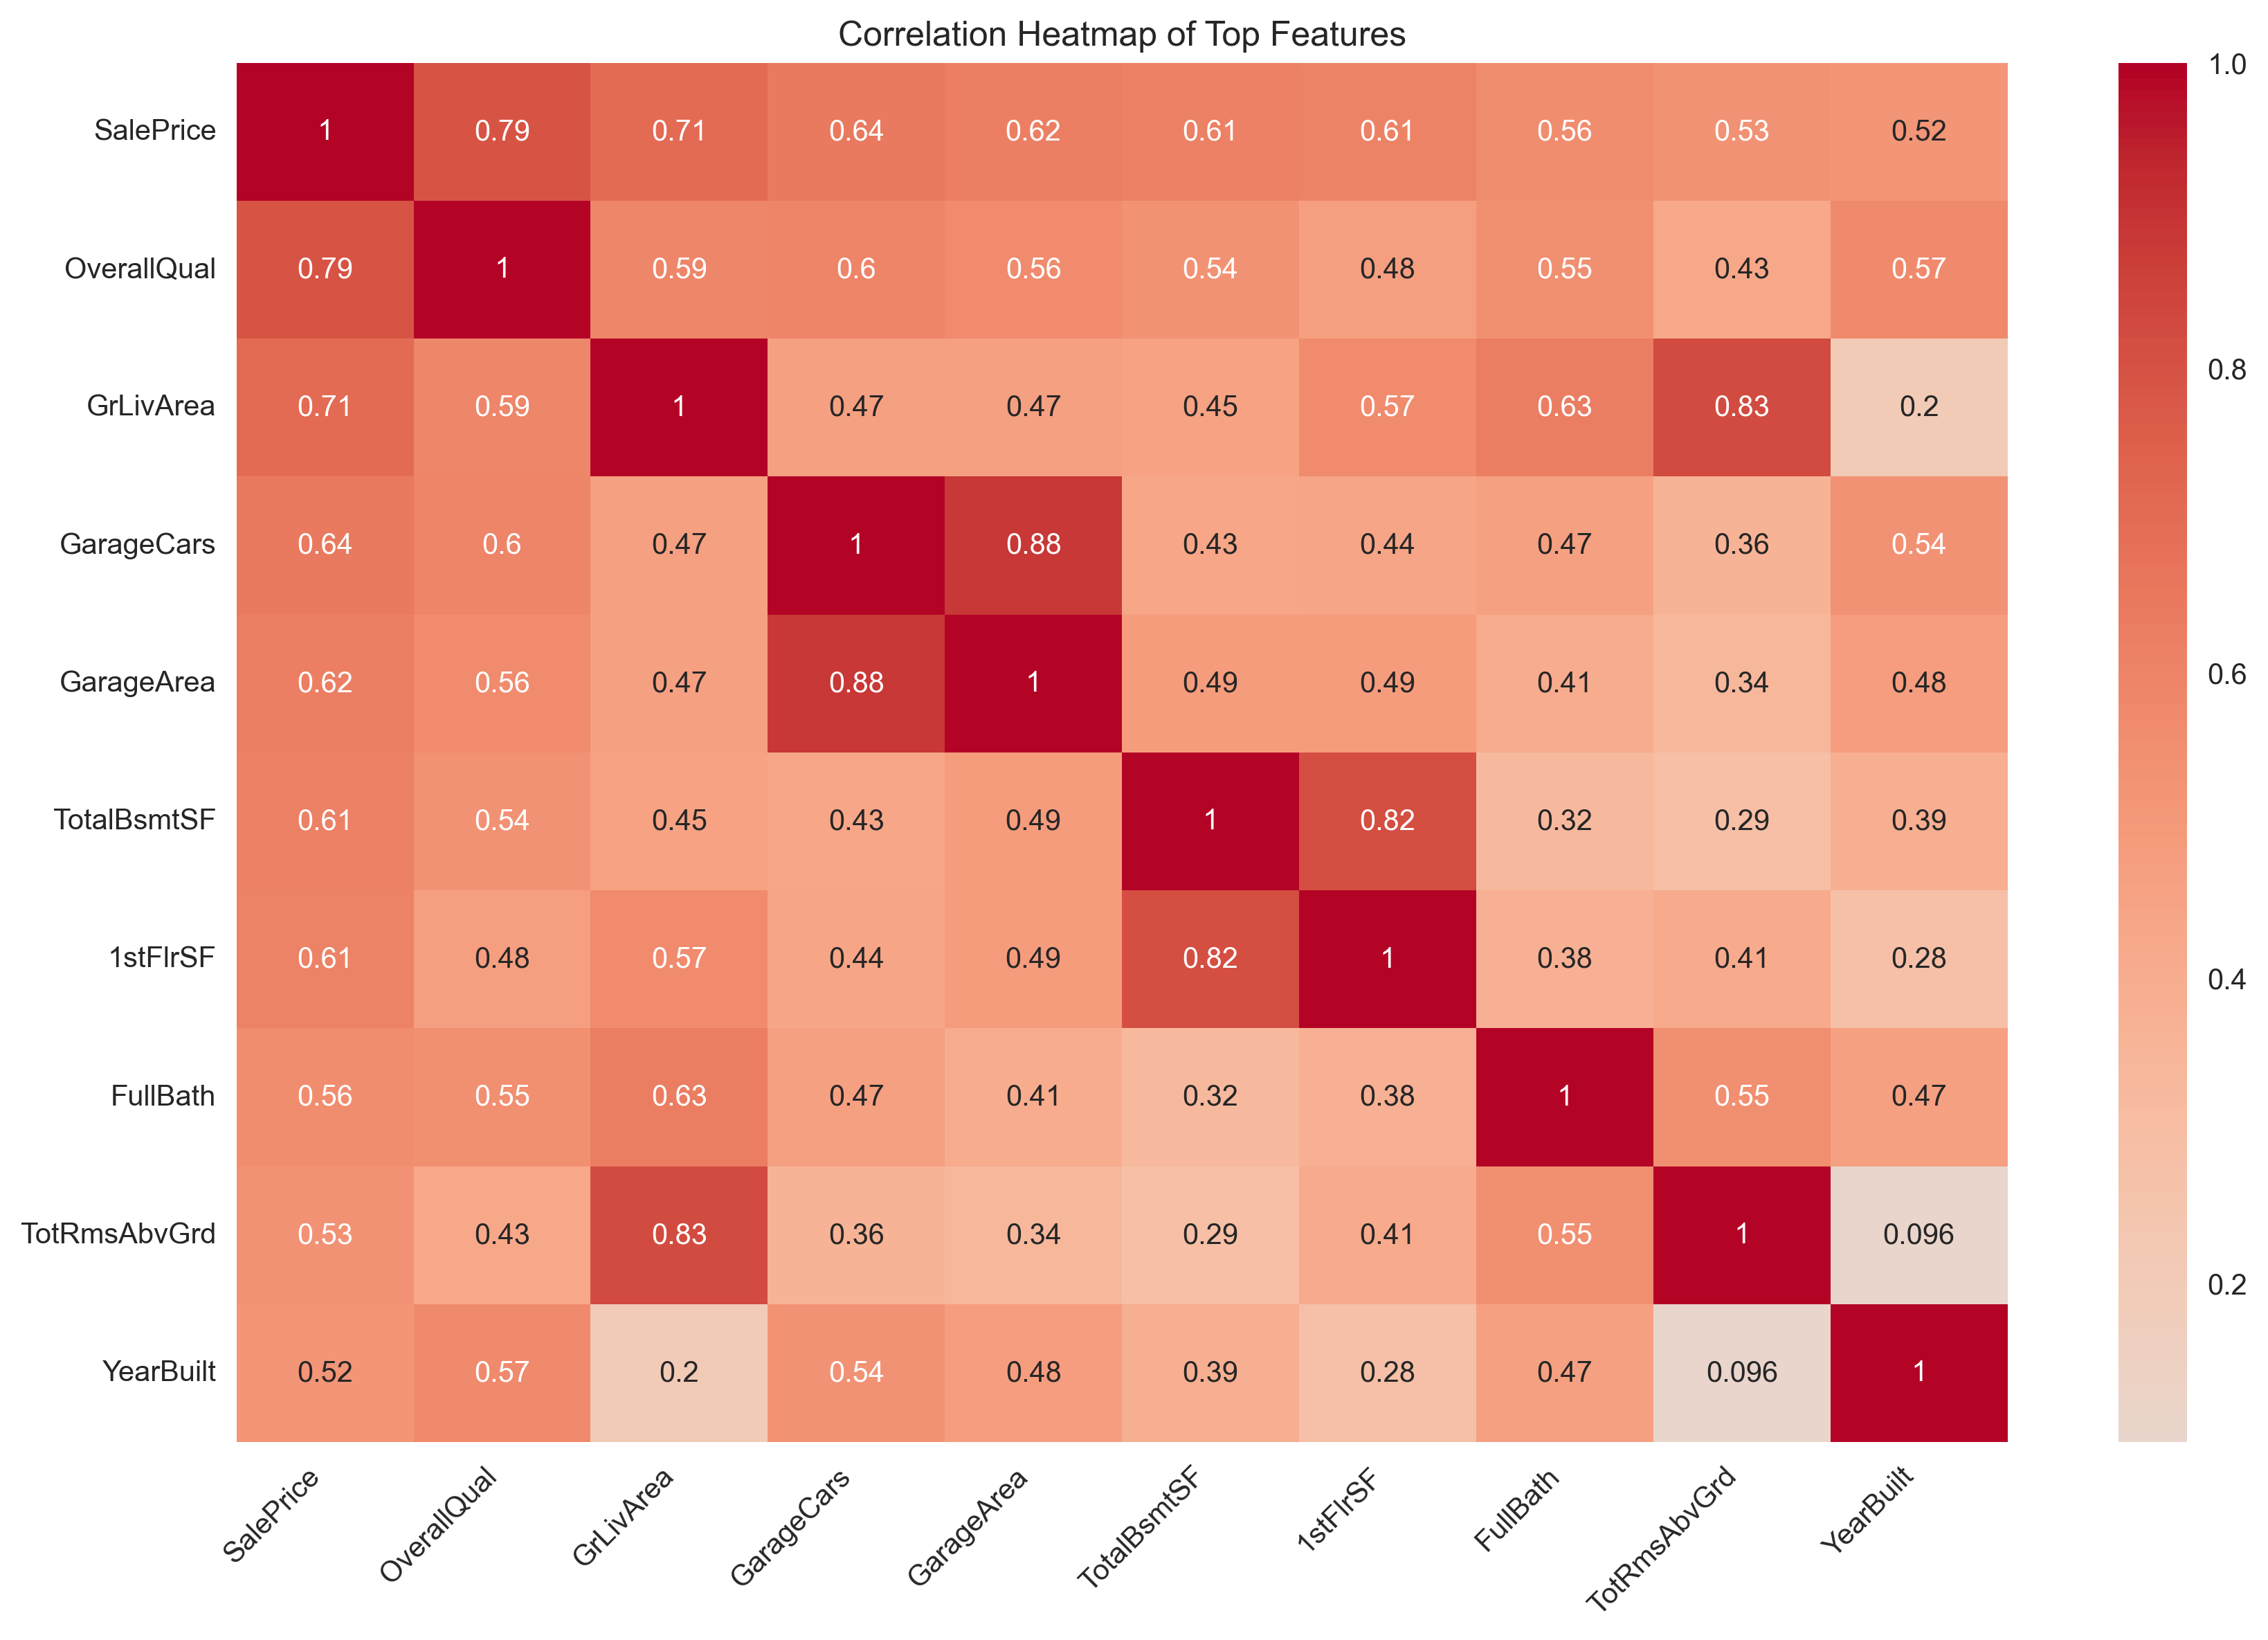
\includegraphics[width=1.0\textwidth]{figures/correlation_matrix.png}
    \caption{Correlation Matrix of Top Features}
    \label{fig:correlation_matrix}
\end{figure}

The correlation analysis reveals:
\begin{itemize}
    \item Overall Quality has the strongest correlation with Sale Price (0.79)
    \item Above Ground Living Area shows strong positive correlation (0.71)
    \item Garage Area and Total Basement SF have moderate correlations (0.62 and 0.61)
    \item Several features show multicollinearity, requiring careful feature selection
\end{itemize}

\subsection{Feature Relationships}
\begin{figure}[H]
    \centering
    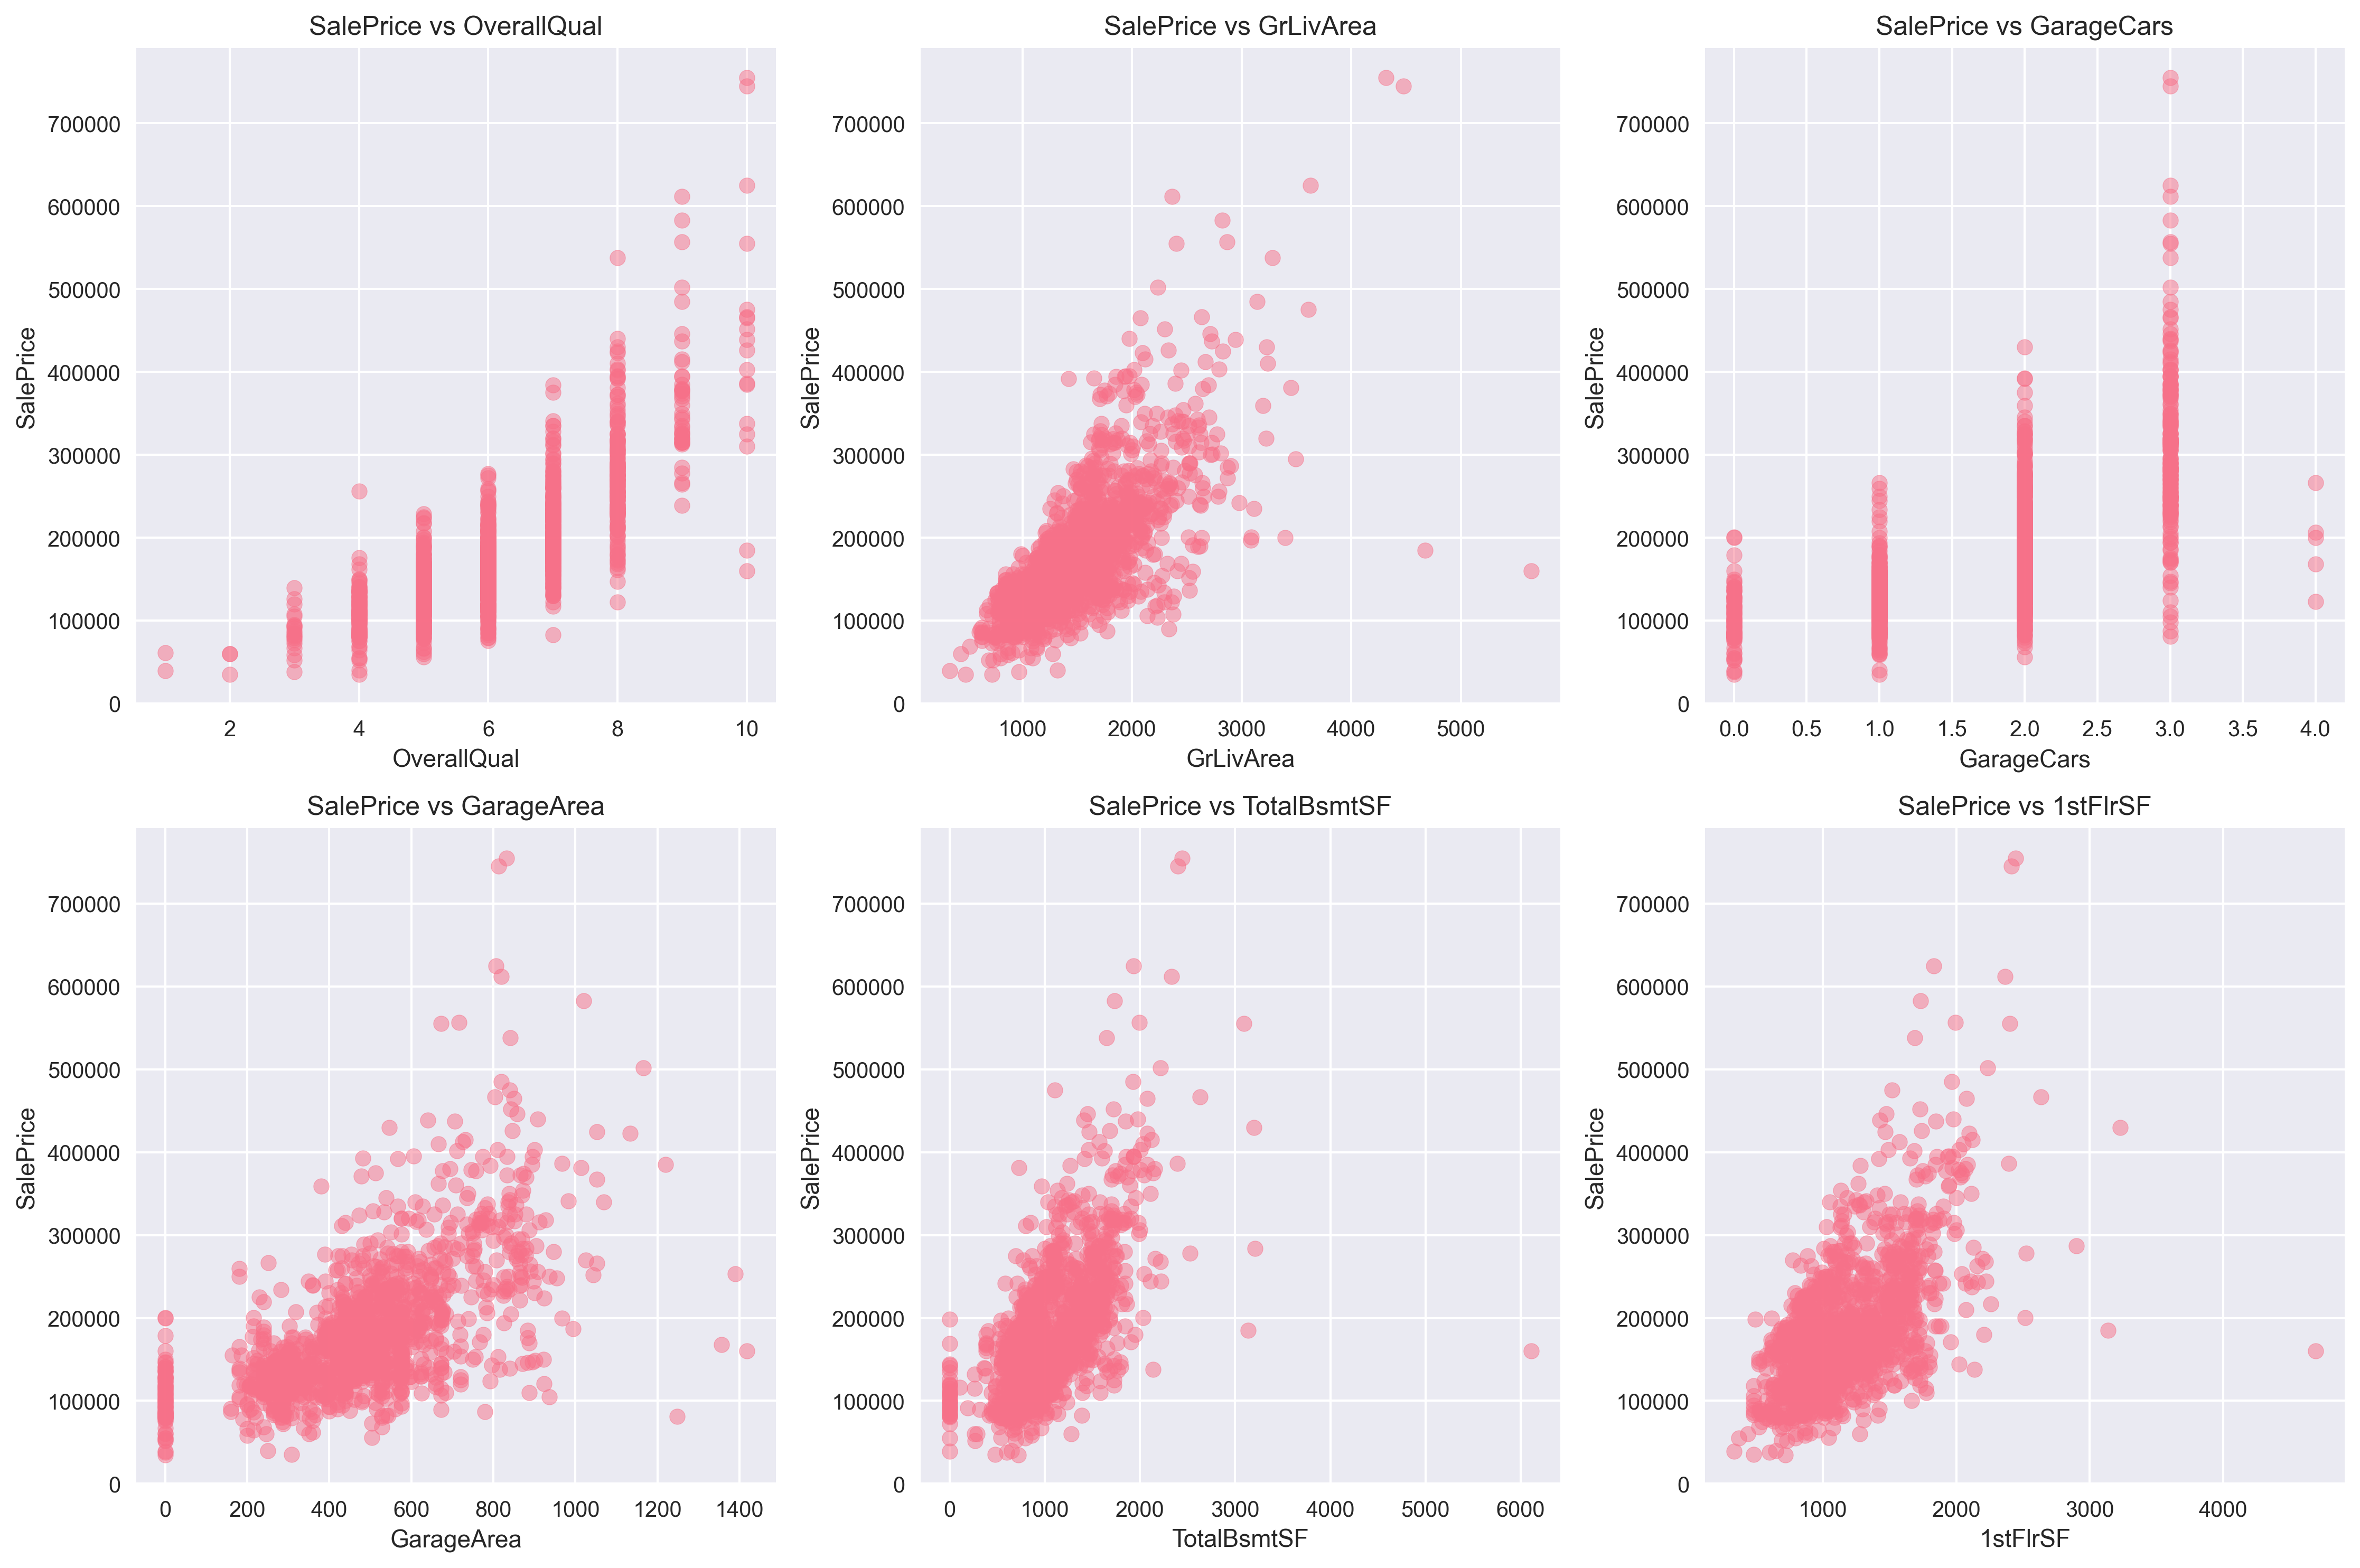
\includegraphics[width=1.0\textwidth]{figures/feature_vs_price.png}
    \caption{Relationships between Key Features and Sale Price}
    \label{fig:feature_price_relation}
\end{figure}

Analysis of feature relationships shows:
\begin{itemize}
    \item Strong linear relationship between Living Area and Price
    \item Overall Quality shows clear step-wise increase in price
    \item Garage Area shows positive correlation but with more scatter
    \item Year Built shows upward trend with newer homes commanding higher prices
\end{itemize}

\section{Categorical Features}
\begin{figure}[H]
    \centering
    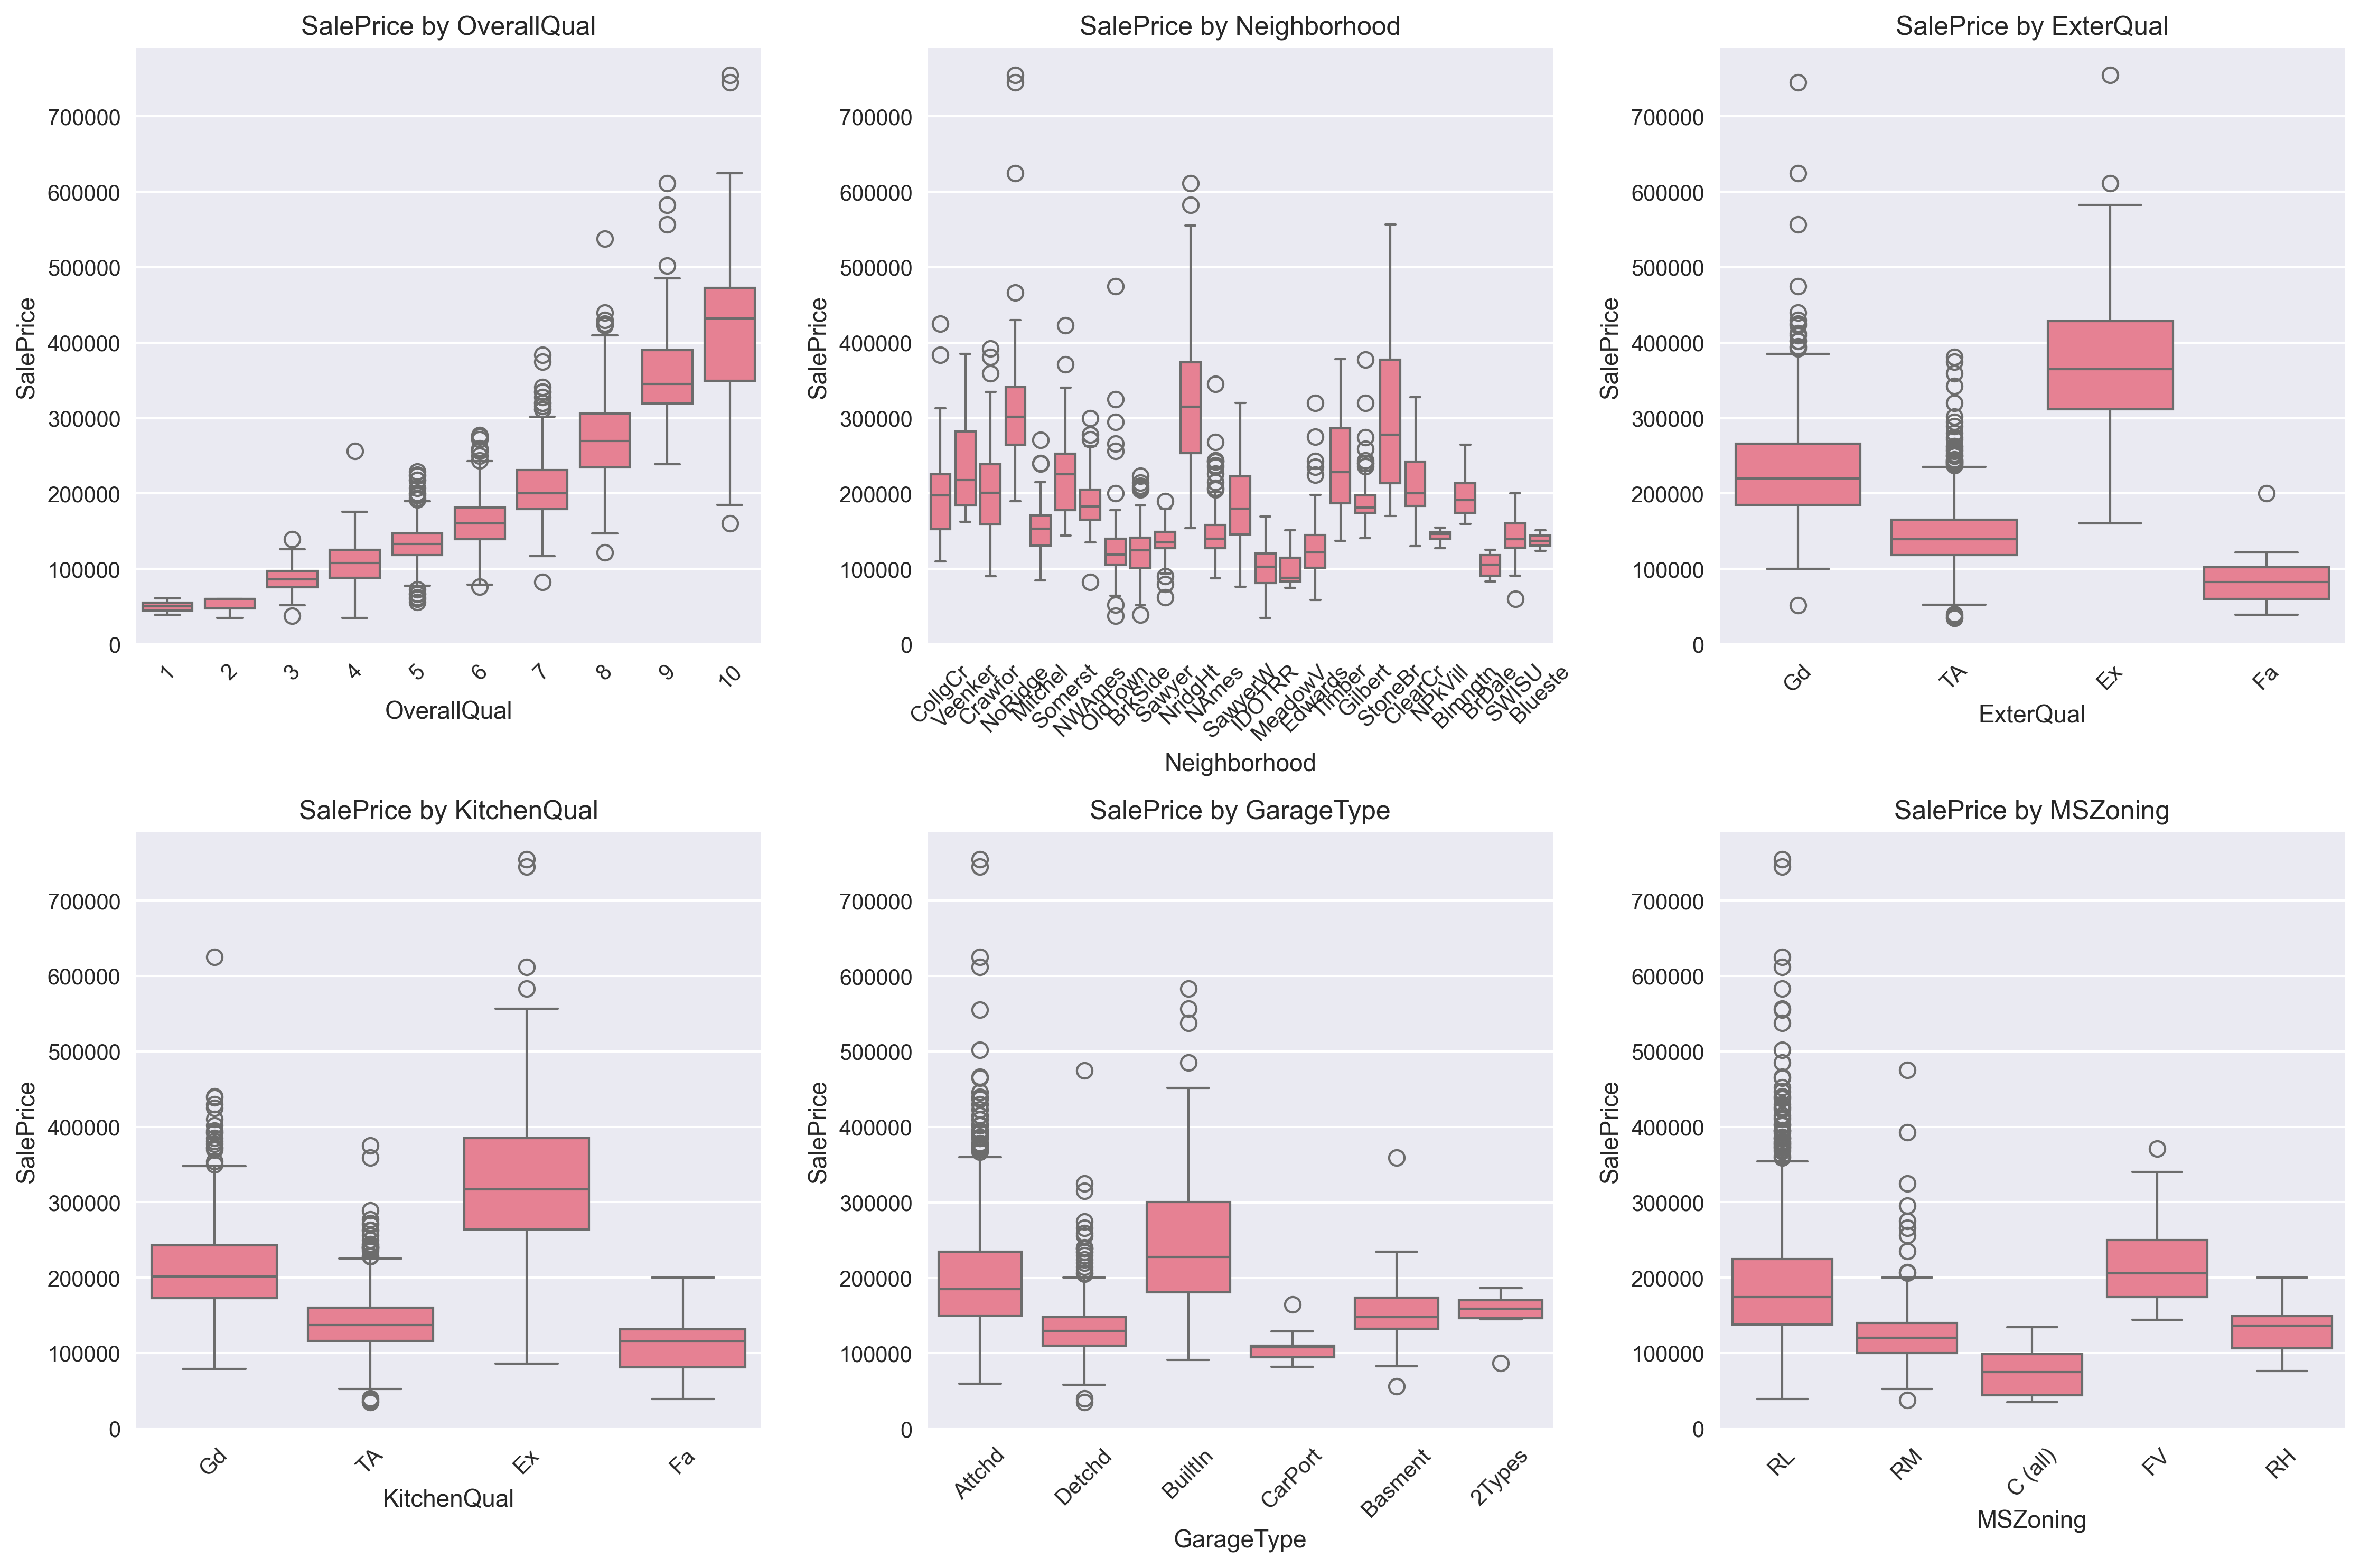
\includegraphics[width=1.0\textwidth]{figures/categorical_features_dist.png}
    \caption{Sale Price Distribution by Categorical Features}
    \label{fig:cat_features_dist}
\end{figure}

Important findings from categorical analysis:
\begin{itemize}
    \item Neighborhood significantly influences price, with NoRidge and NridgHt commanding highest prices
    \item Overall Quality shows clear price progression from 1 to 10
    \item Kitchen and Exterior Quality ratings strongly correlate with price
    \item Zoning categories show distinct price ranges, with RL (Residential Low Density) being most common
\end{itemize}

\section{Outlier Analysis}
\begin{figure}[H]
    \centering
    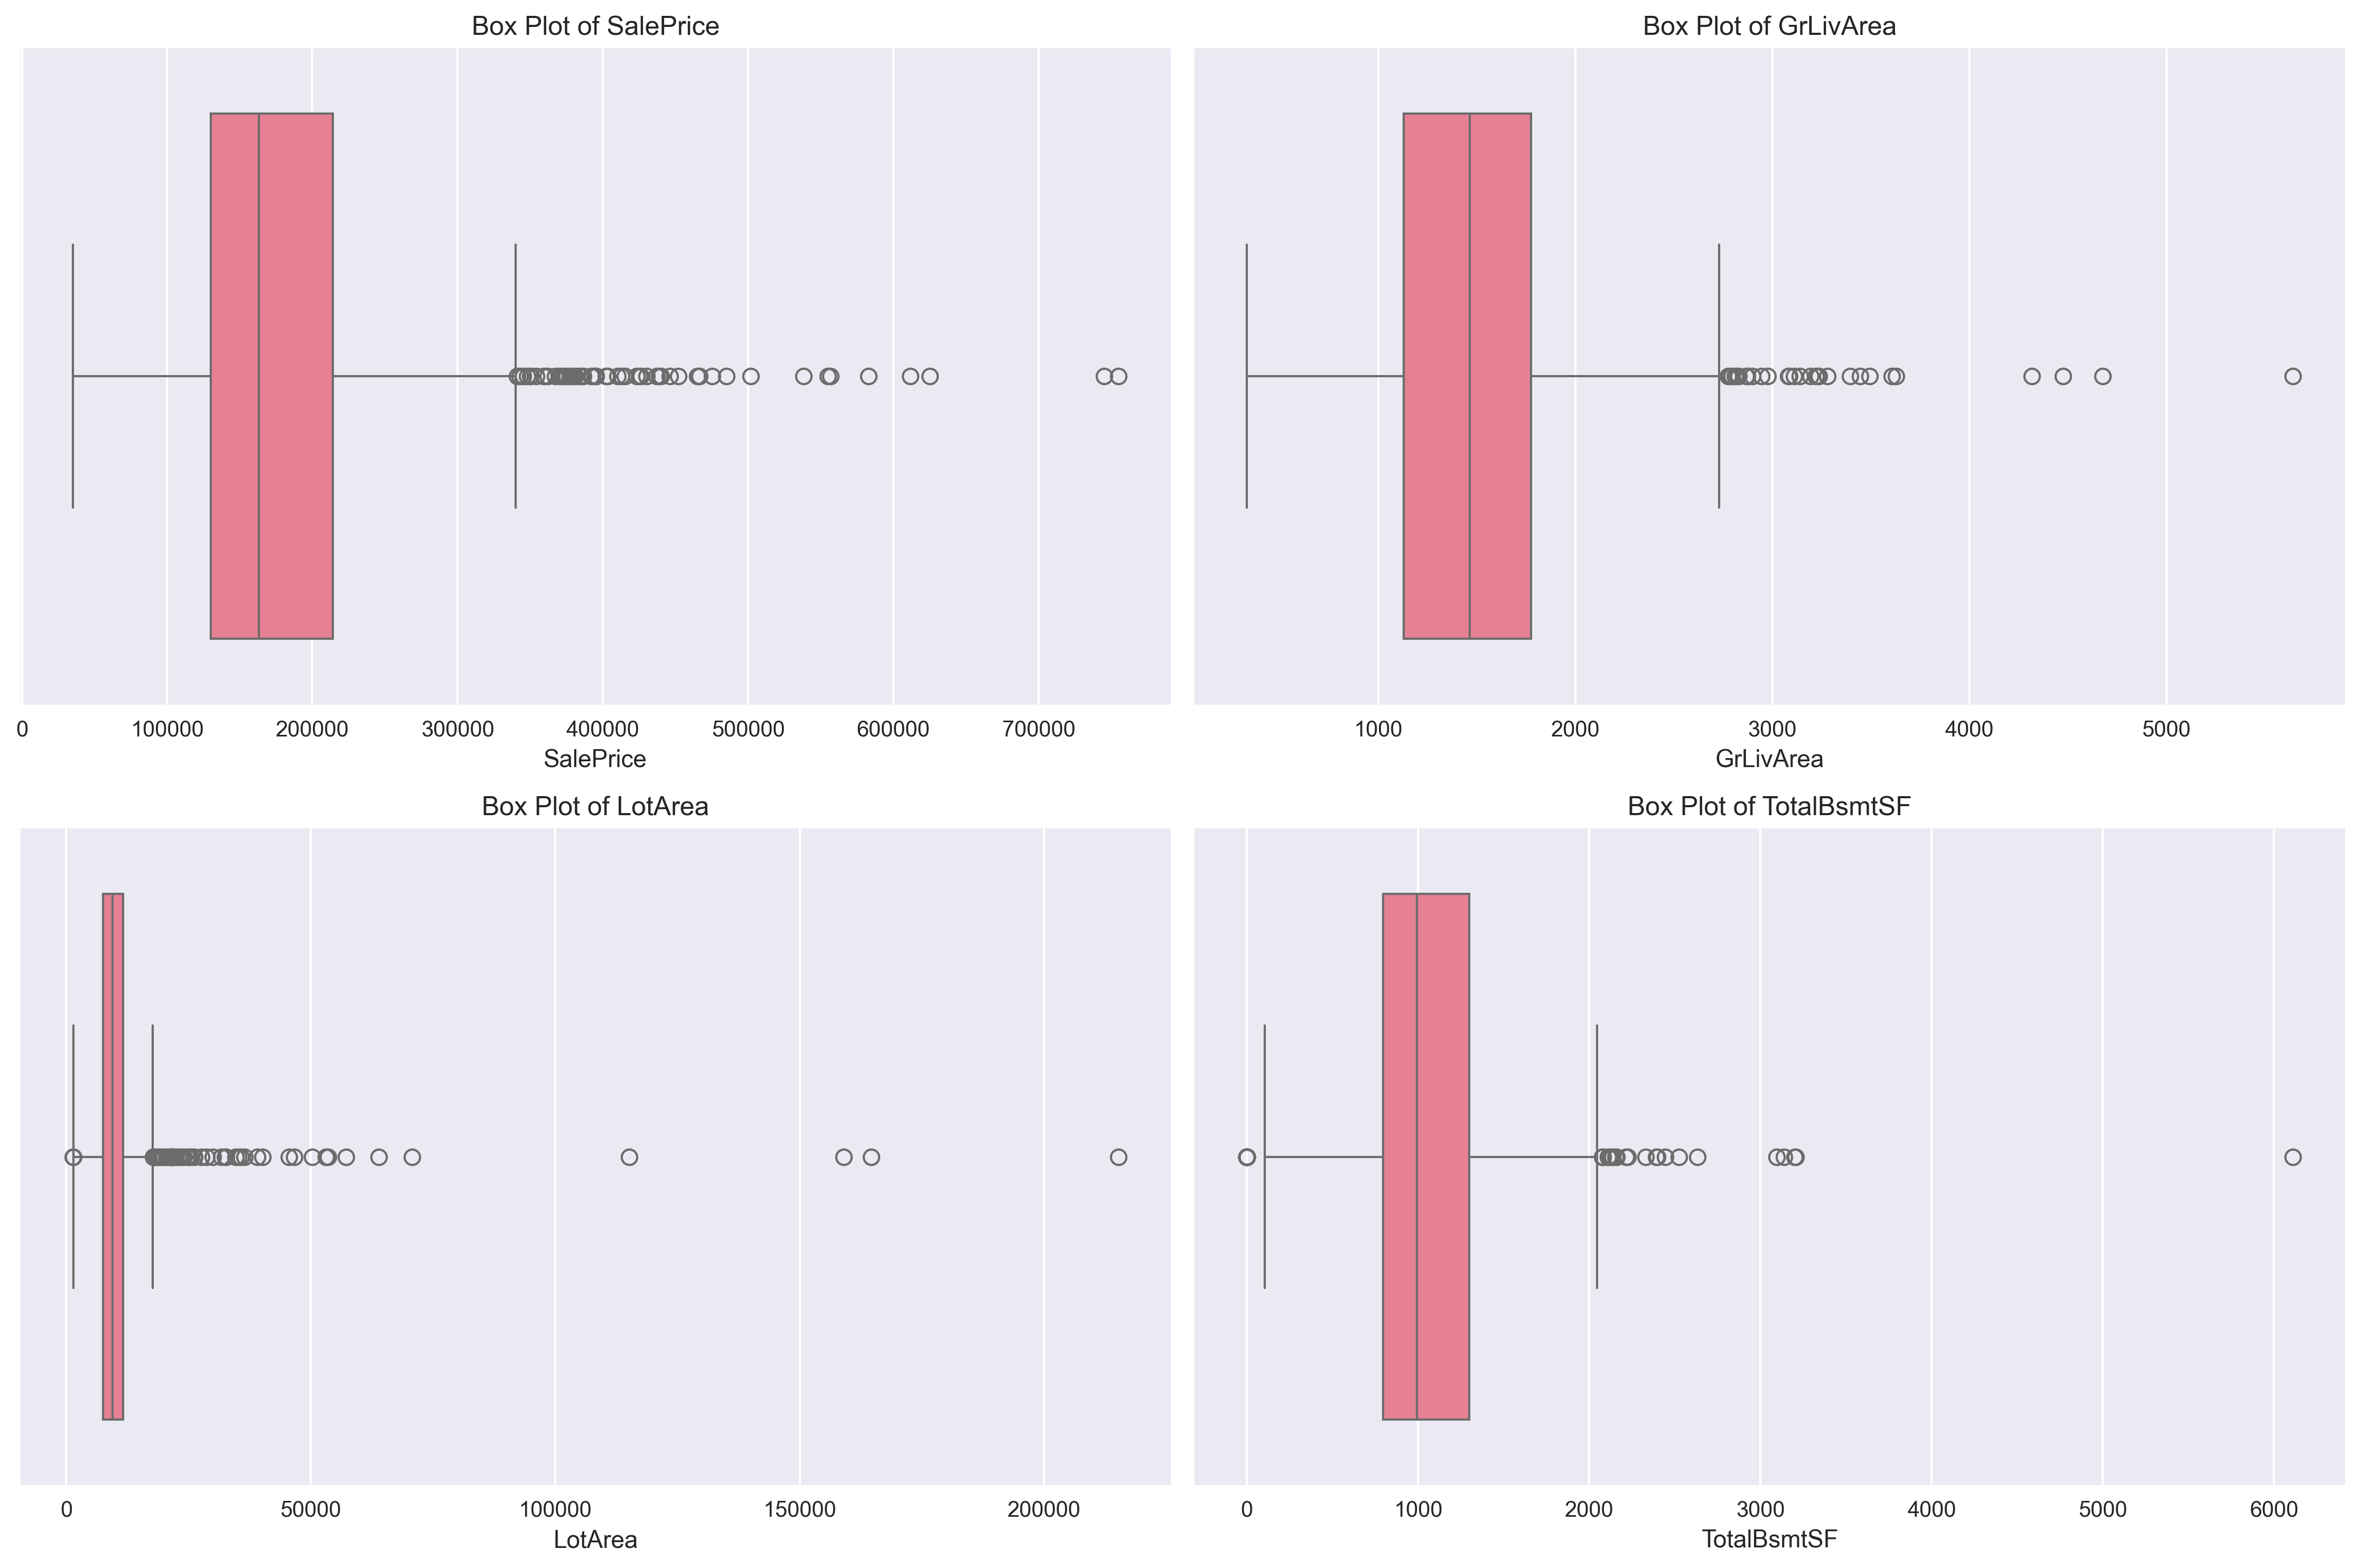
\includegraphics[width=1.0\textwidth]{figures/outliers_boxplot.png}
    \caption{Boxplots Showing Outliers in Key Features}
    \label{fig:outliers}
\end{figure}

Outlier detection reveals:
\begin{itemize}
    \item Several properties with extremely high sale prices (>2.5 IQR)
    \item GrLivArea has notable outliers above 4,000 sq ft
    \item Lot Area shows extreme outliers, with some lots significantly larger than typical
    \item Total Basement SF outliers align with larger homes
\end{itemize}

\section{Feature Importance}
\begin{figure}[H]
    \centering
    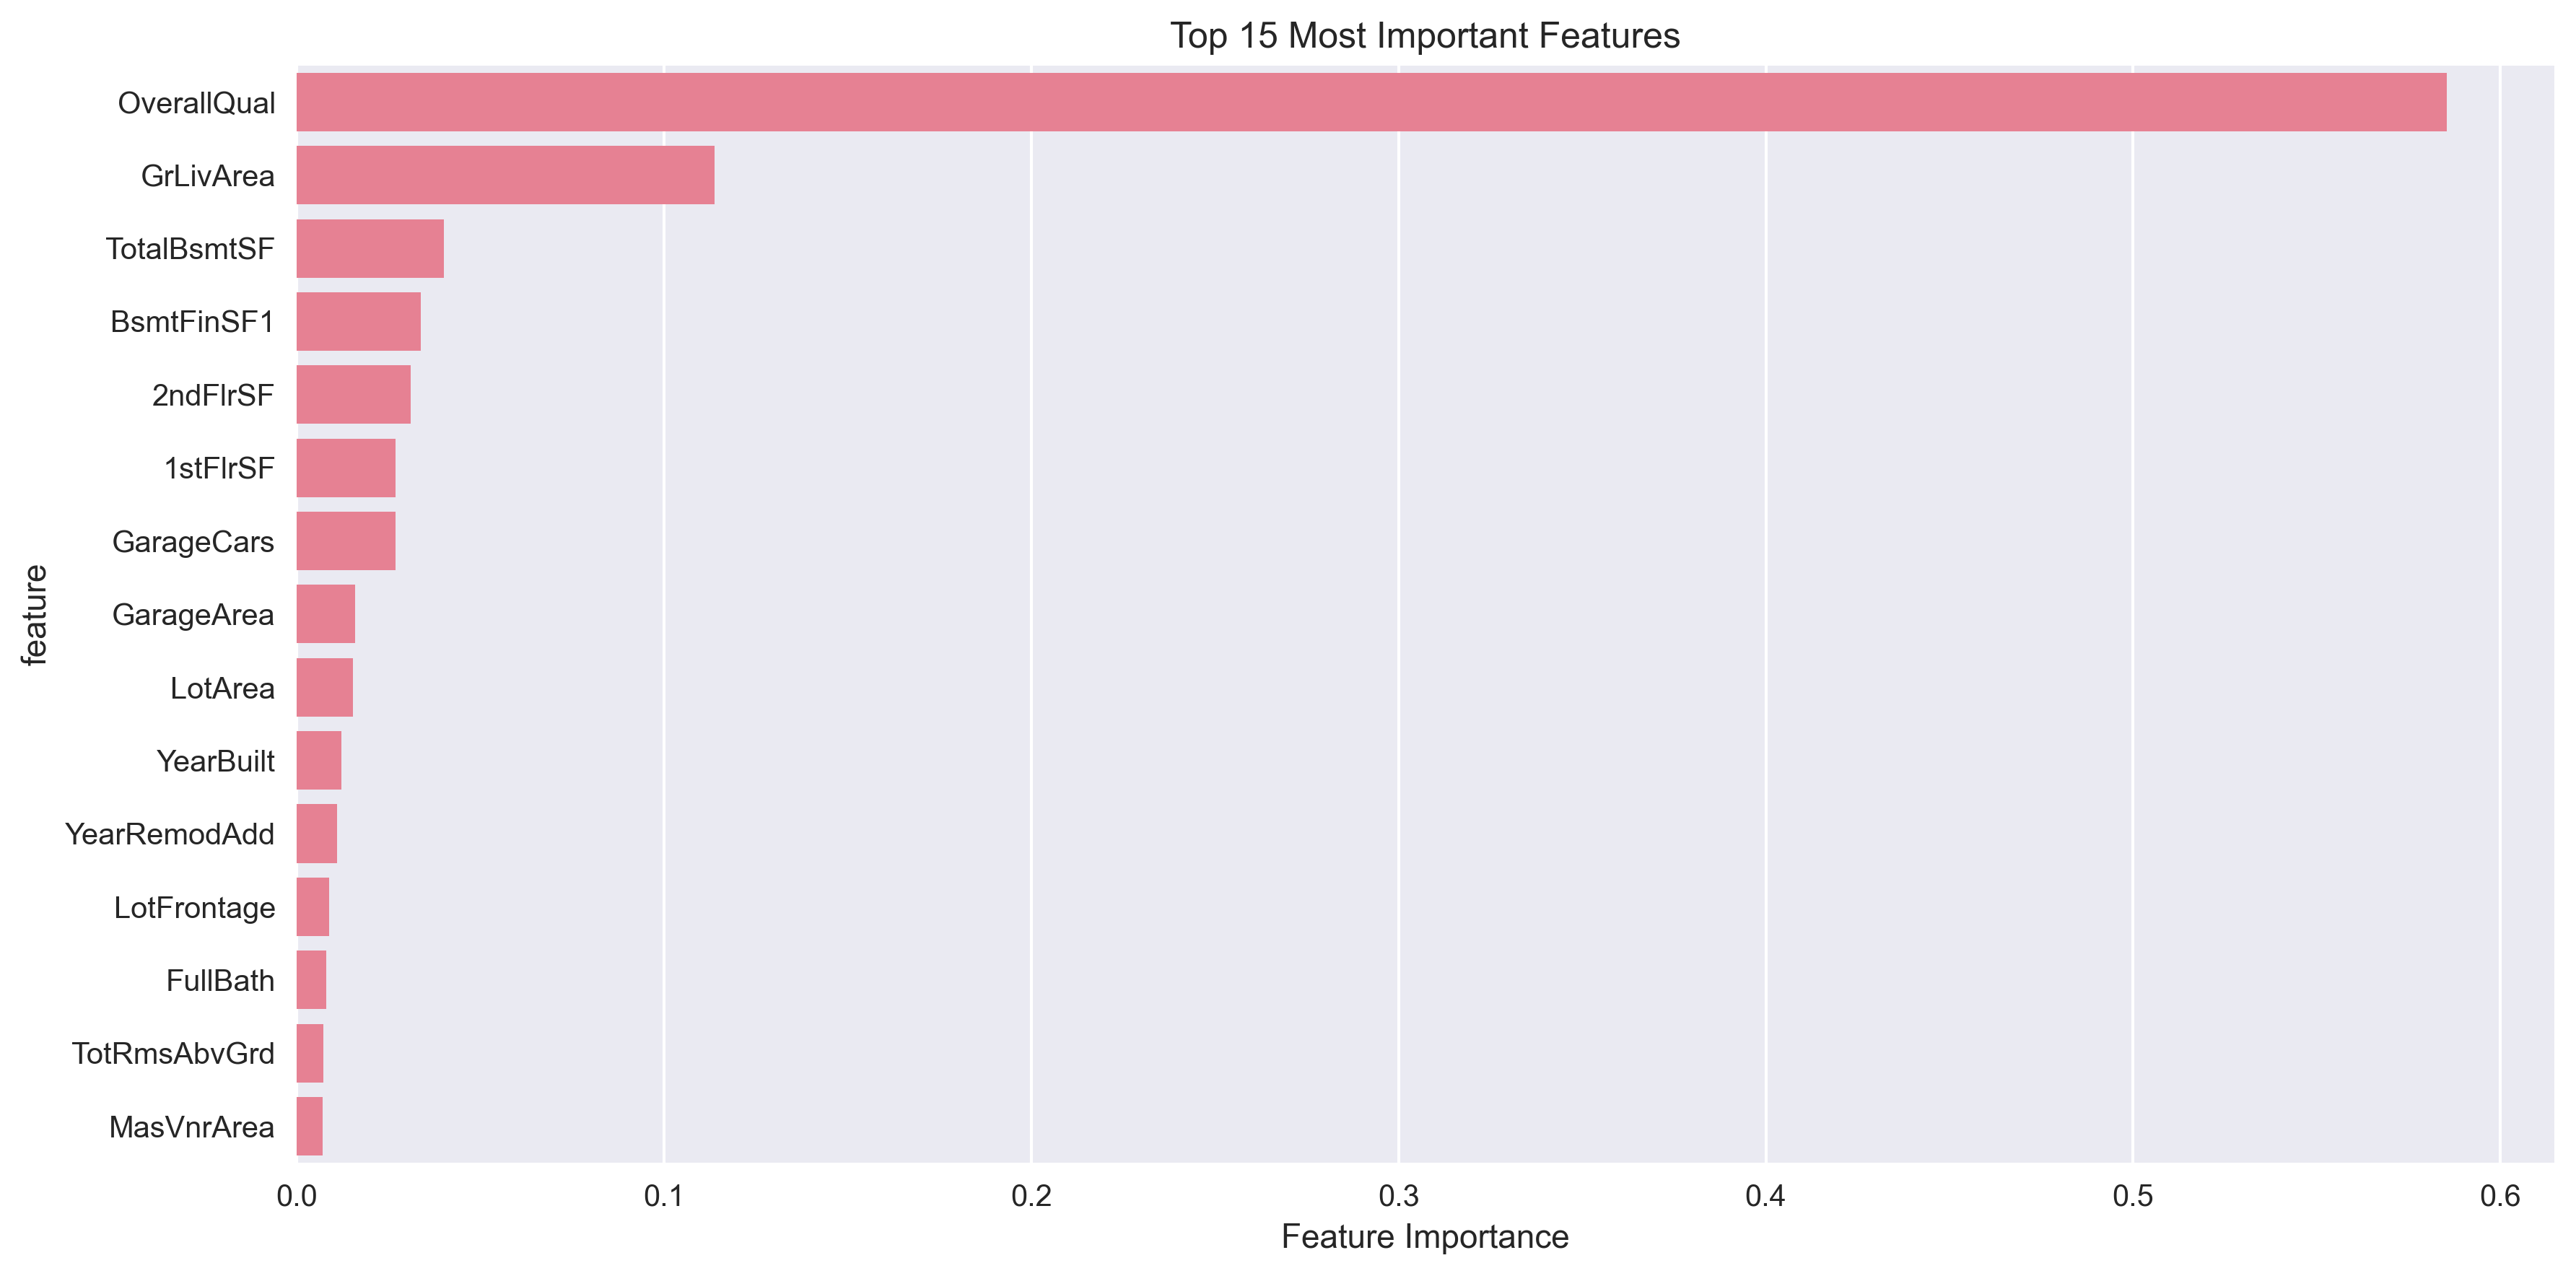
\includegraphics[width=1.0\textwidth]{figures/feature_importance.png}
    \caption{Random Forest Feature Importance Analysis}
    \label{fig:feature_importance}
\end{figure}

The Random Forest analysis identifies key predictors:
\begin{itemize}
    \item Overall Quality emerges as the most important feature
    \item Ground Living Area is the second most important predictor
    \item Year Built and Total Basement SF show significant importance
    \item Garage Area and First Floor SF also contribute meaningfully
\end{itemize}

\section{Key Findings and Recommendations}
Based on the comprehensive EDA, we recommend:
\begin{itemize}
    \item Log transformation of Sale Price and some size-related features
    \item Careful handling of outliers, especially in GrLivArea and Lot Area
    \item Feature engineering combining quality ratings
    \item Neighborhood-based feature engineering
    \item Treatment of missing values based on domain context
    \item Consideration of interaction terms between quality and size features
\end{itemize}

These insights will guide our modeling approach, particularly in:
\begin{itemize}
    \item Feature selection and engineering
    \item Choice of regression techniques
    \item Handling of non-linear relationships
    \item Treatment of categorical variables
\end{itemize}

% Chapter 3: Modeling Approaches
\chapter{Modeling Approaches}

\section{Introduction}
This chapter presents four different modeling approaches for predicting house prices in the Ames Housing dataset:
\begin{itemize}
    \item Ridge Regression (L2 regularization) with 10-fold cross validation
    \item Lasso Regression (L1 regularization) with 10-fold cross validation
    \item Random Forest Regression with 10-fold cross validation
    \item PyTorch Neural Network with 10-fold cross validation
\end{itemize}

Each model offers unique advantages and characteristics in handling the complexities of house price prediction.
For this analysis, we excluded variables with high proportions of missing values: "PoolQC", "MiscFeature", "Alley", "Fence", "MasVnrType", and "FireplaceQu". For remaining missing values, we applied imputation using mean values for numerical features and most frequent values for categorical features.

\section{Ridge Regression}
Ridge regression addresses multicollinearity by adding an L2 penalty term to the loss function. This approach is particularly useful for our dataset given the high correlations observed between various features.

\subsection{Hyperparameter Tuning}

\begin{figure}[H]
    \centering
    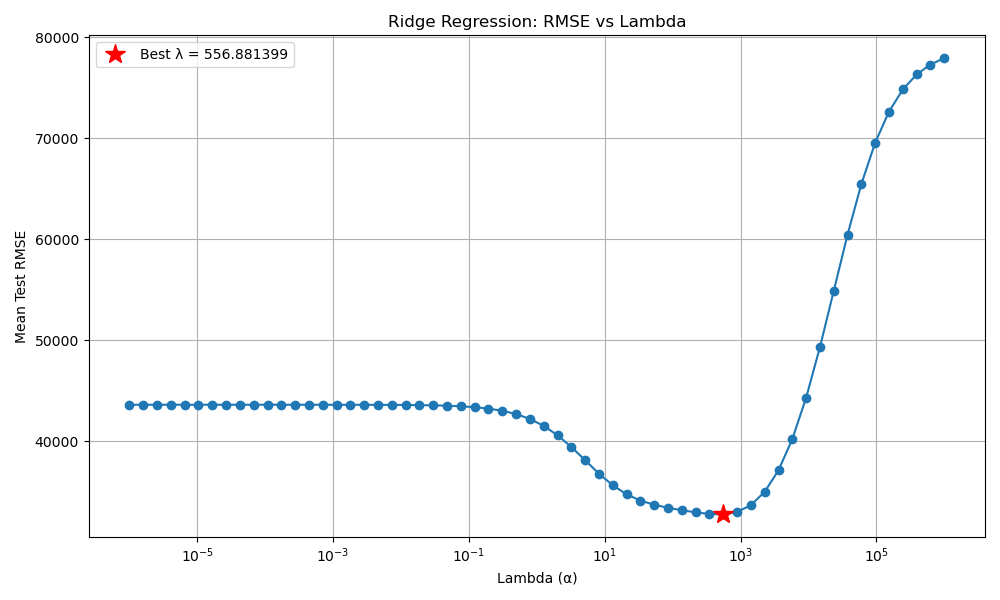
\includegraphics[width=1.0\textwidth]{figures/ridge_lambda_vs_rmse.png}
    \caption{Effect of Ridge Regularization Parameter on Model Performance}
    \label{fig:ridge_lambda}
\end{figure}

The analysis of different lambda values reveals:
\begin{itemize}
    \item Optimal lambda value found through 10-fold cross-validation
    \item Model performance initially improves with increased regularization
    \item Excessive regularization leads to underfitting, as shown by increasing RMSE
    \item Clear bias-variance tradeoff demonstrated in the U-shaped error curve
\end{itemize}

\subsection{Feature Importance}
\begin{figure}[H]
    \centering
    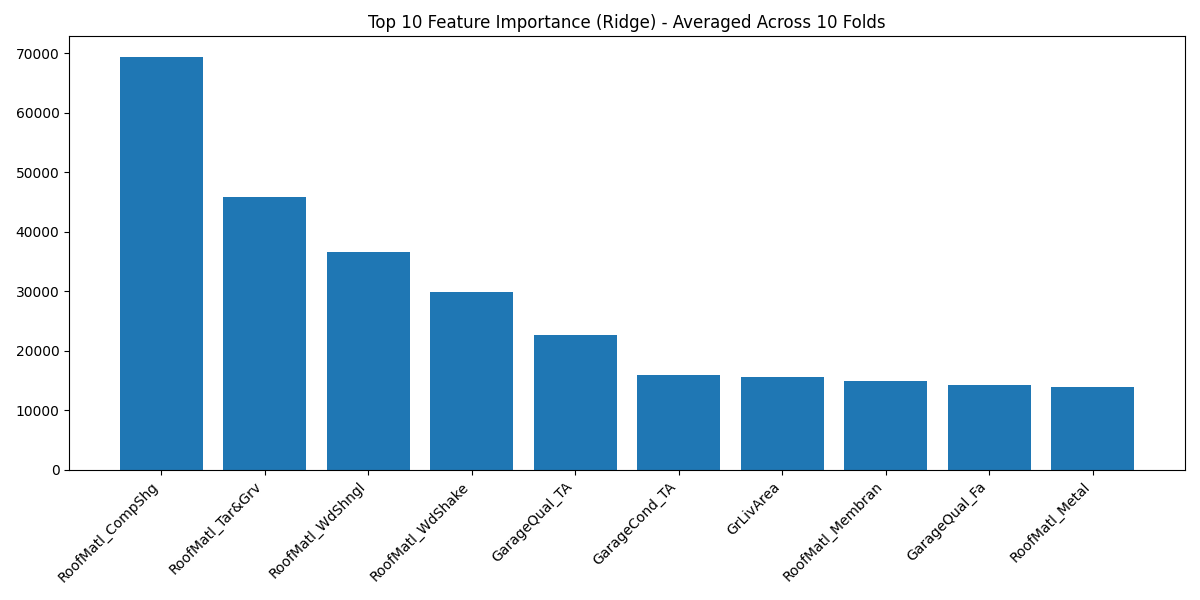
\includegraphics[width=1.0\textwidth]{figures/ridge_feature_importance.png}
    \caption{Top 10 Features by Importance in Ridge Regression}
    \label{fig:ridge_importance}
\end{figure}

Key findings from Ridge regression:
\begin{itemize}
    \item Overall Quality remains the strongest predictor
    \item Living Area shows significant impact
    \item Age-related features (Year Built, Year Remodeled) demonstrate importance
    \item Location factors contribute meaningfully to predictions
\end{itemize}

\section{Lasso Regression}
Lasso regression performs both regularization and feature selection through L1 penalty, potentially reducing model complexity by eliminating less important features.

\subsection{Parameter Optimization}
\begin{figure}[H]
    \centering
    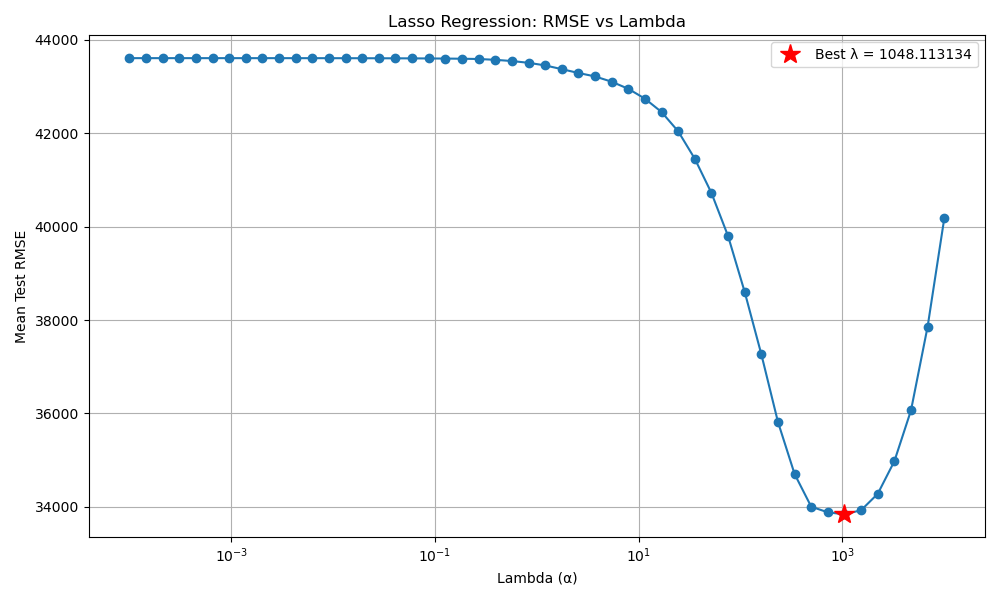
\includegraphics[width=1.0\textwidth]{figures/lasso_lambda_vs_rmse.png}
    \caption{Impact of Lasso Regularization Parameter on RMSE}
    \label{fig:lasso_lambda}
\end{figure}

The lambda parameter analysis shows:
\begin{itemize}
    \item Optimal lambda value identified through 10-fold cross-validation
    \item Feature selection becomes more aggressive at higher lambda values
    \item Similar U-shaped error curve to Ridge, demonstrating bias-variance tradeoff
    \item Performance deteriorates rapidly with excessive regularization
\end{itemize}

\subsection{Feature Selection}
\begin{figure}[H]
    \centering
    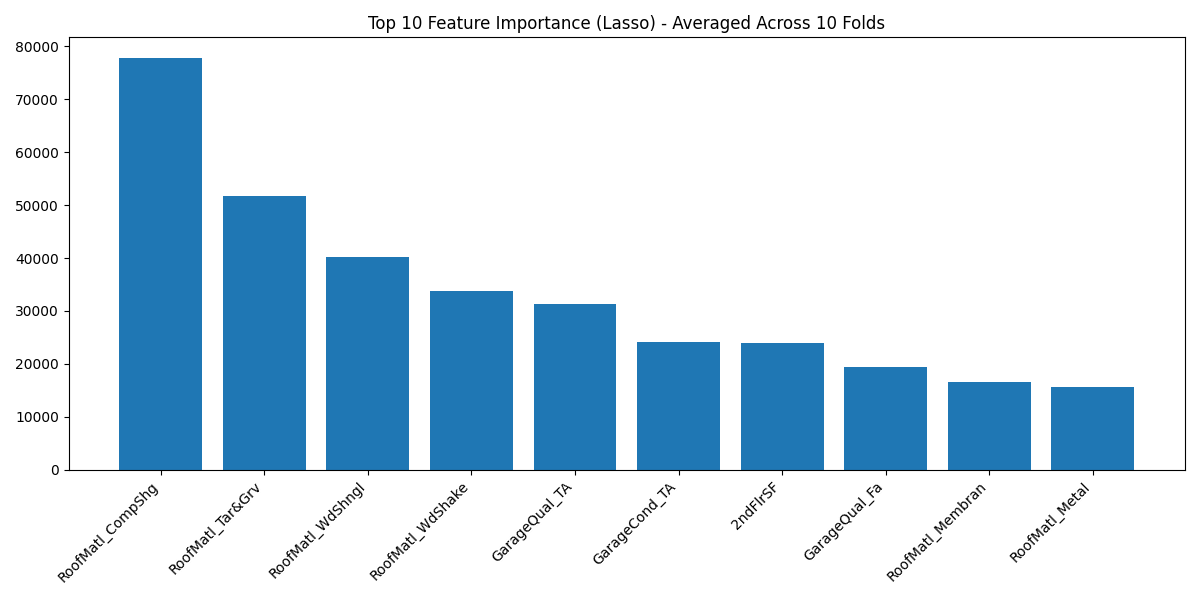
\includegraphics[width=1.0\textwidth]{figures/lasso_feature_importance.png}
    \caption{Top 10 Features by Importance from Lasso Regression}
    \label{fig:lasso_importance}
\end{figure}

Lasso regression reveals:
\begin{itemize}
    \item Automatic feature selection through coefficient shrinkage
    \item Identification of most crucial price determinants
    \item Sparse feature representation for improved interpretability
    \item Consistency with Ridge regression in key feature identification
\end{itemize}

\section{Random Forest Regression}
Random Forest is an ensemble method that leverages multiple decision trees to capture complex non-linear relationships and interactions between features.

\subsection{Model Implementation}
Our Random Forest implementation included the following components:
\begin{itemize}
    \item Ensemble of 100 decision trees, each trained on bootstrap samples
    \item Feature selection at each split using a random subset of features
    \item Maximum depth controlled to prevent overfitting
    \item 10-fold cross-validation for robust performance evaluation
\end{itemize}

Random Forest regression offers several advantages for this housing price prediction task:
\begin{itemize}
    \item Handles non-linear relationships without explicit transformation
    \item Naturally incorporates feature interactions
    \item Robust to outliers and non-normally distributed data
    \item Provides built-in feature importance measures
    \item Less sensitive to hyperparameter tuning than linear models
\end{itemize}

\subsection{Feature Importance}
One of the key benefits of Random Forest is its ability to compute feature importance. The algorithm calculates importance based on how much each feature decreases impurity when used in tree splits. The model identified several key predictors:

\begin{itemize}
    \item Overall Quality remained the dominant feature
    \item Ground Living Area showed high importance
    \item Year Built and neighborhood variables demonstrated strong impact
    \item Lot Area and basement features showed moderate importance
\end{itemize}

\subsection{Performance Analysis}
The Random Forest model achieved excellent predictive performance:
\begin{itemize}
    \item 10-fold CV RMSE: 29,042.51
    \item Test RMSE: 29,032.17
    \item Test R²: 0.8901
\end{itemize}

This performance positions Random Forest as one of the top-performing models in our comparison, with better metrics than the linear models in most cases. The algorithm's ability to capture non-linear relationships and interactions between features proved beneficial for this dataset.

\section{Neural Network Regression}
A deep learning approach using neural networks offers the potential to capture complex, non-linear relationships in the data.

\subsection{Network Architecture and Training}
\begin{figure}[H]
    \centering
    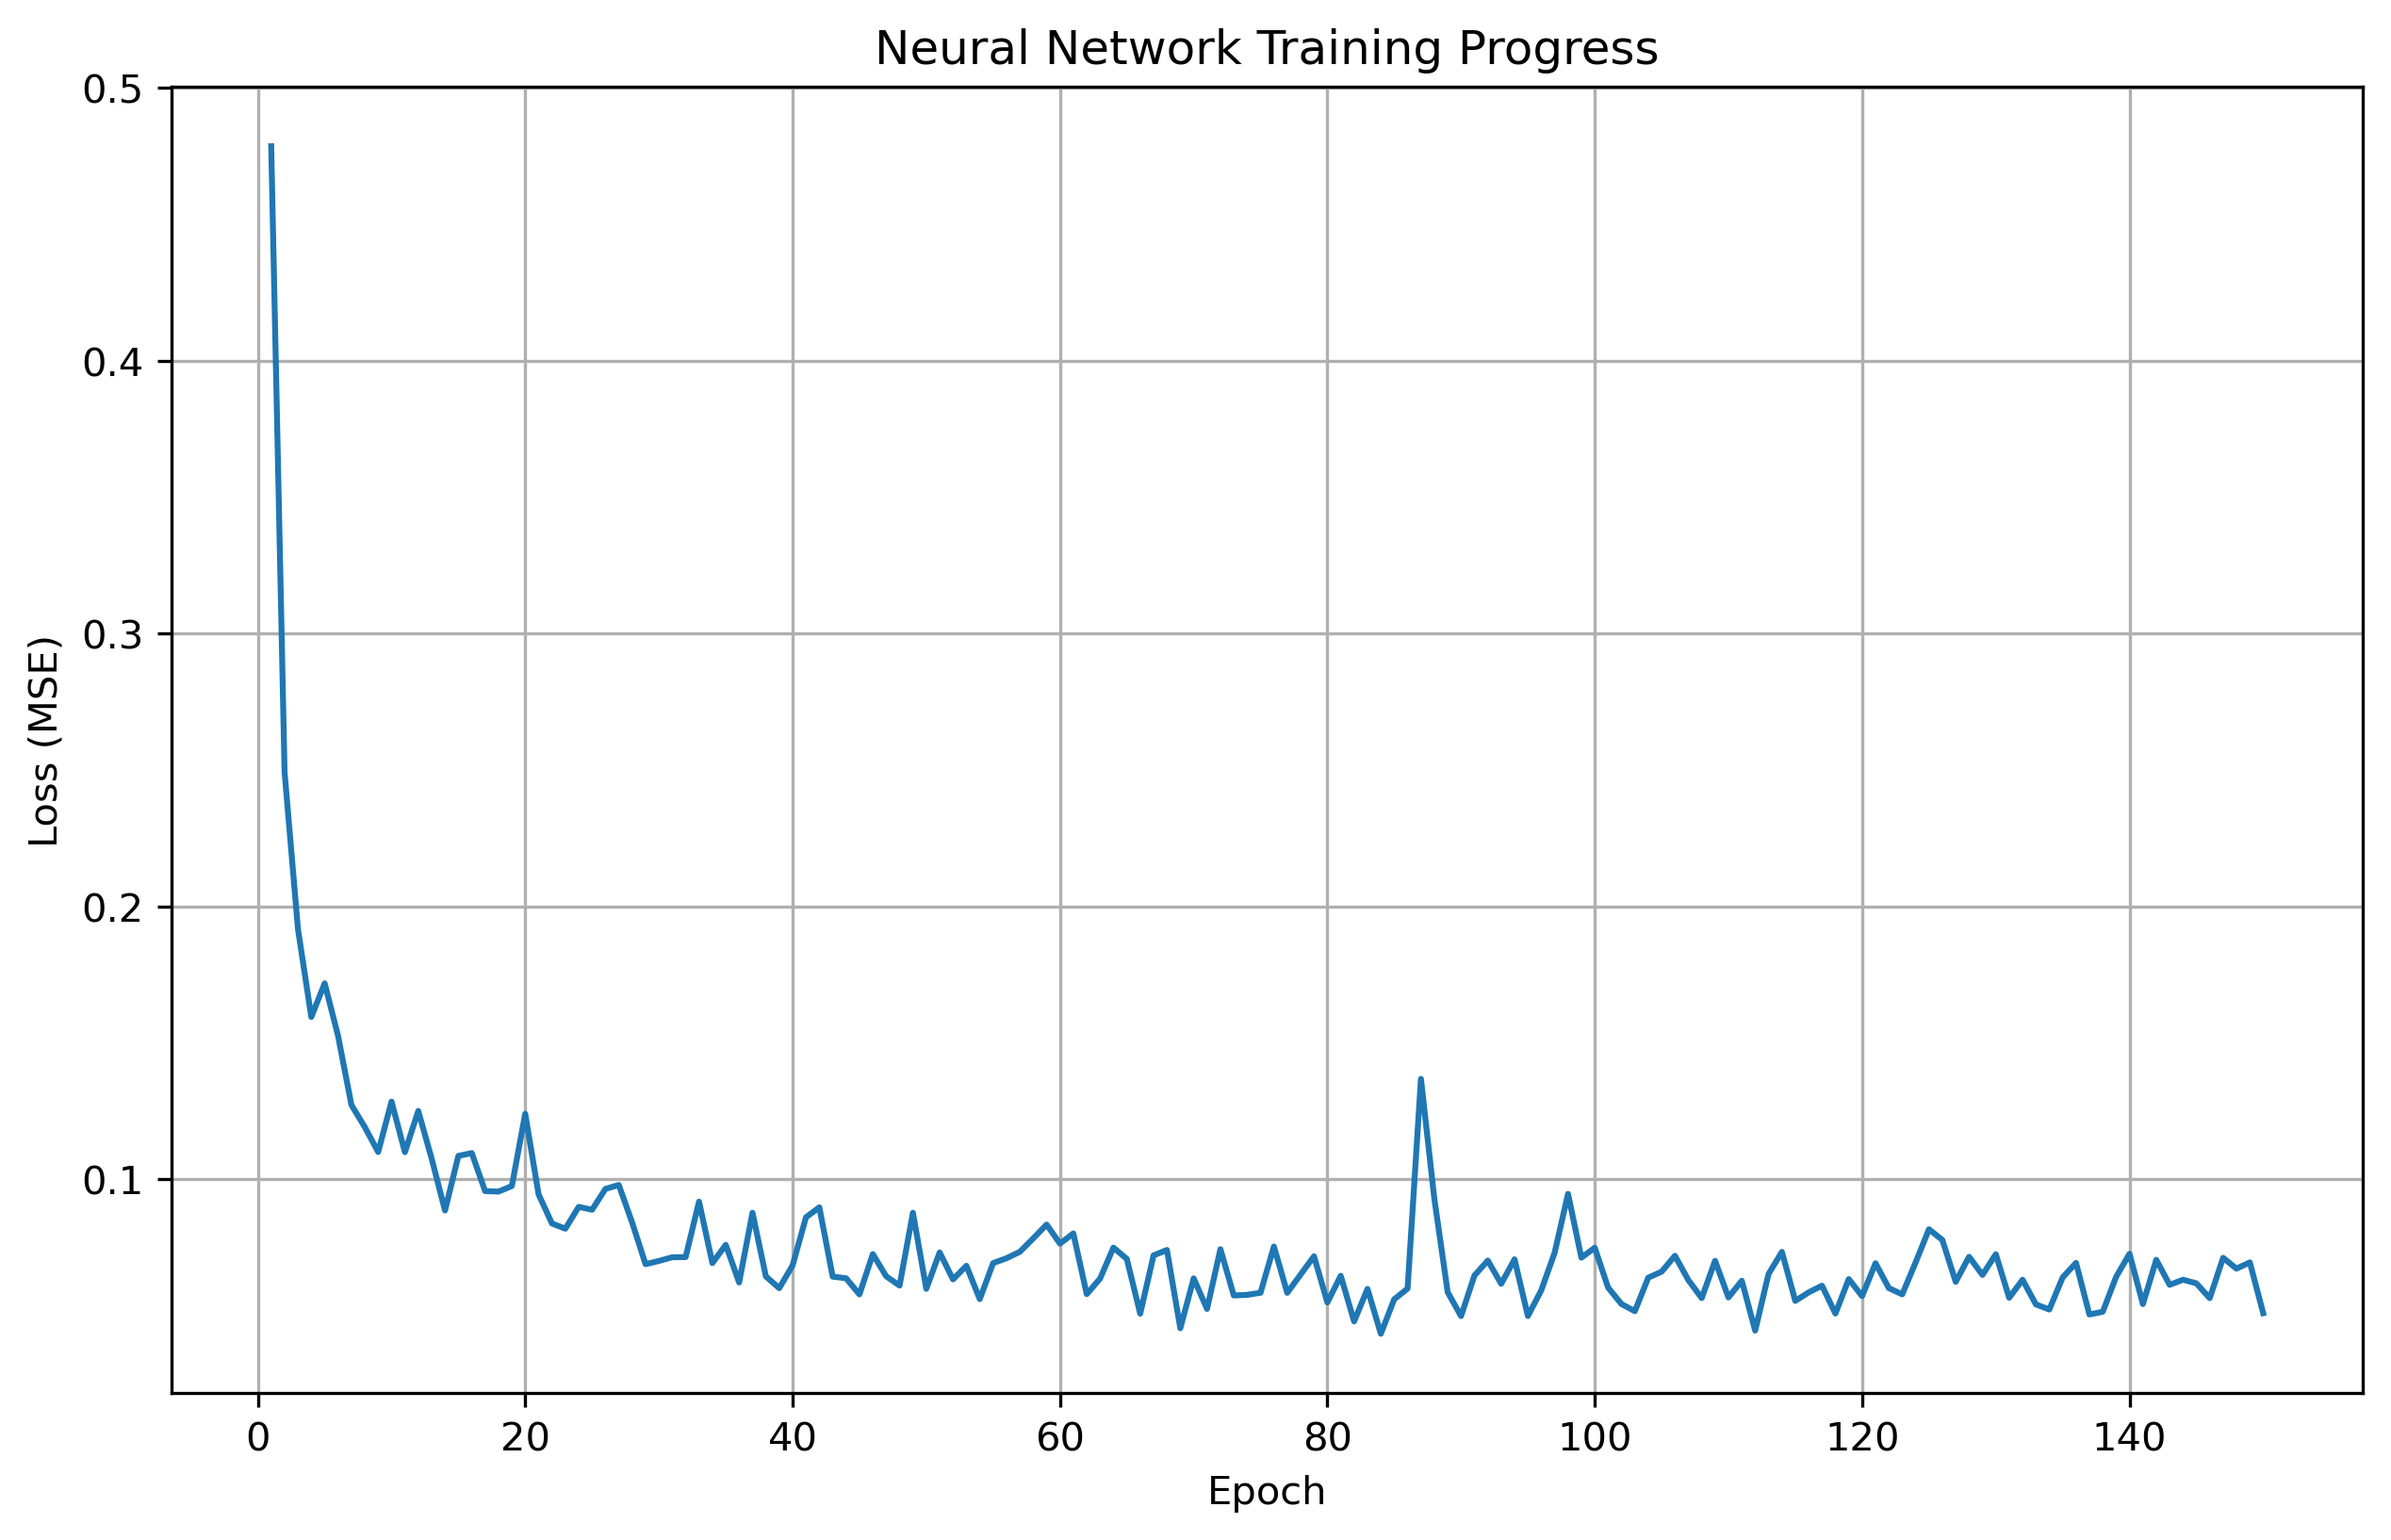
\includegraphics[width=1.0\textwidth]{figures/neural_network_training.png}
    \caption{Neural Network Training Progress}
    \label{fig:nn_training}
\end{figure}

The neural network implementation:
\begin{itemize}
    \item Uses a deeper architecture with 4 layers (128→64→32→1)
    \item Incorporates batch normalization after each hidden layer
    \item Employs ReLU activation and dropout (0.2) for regularization
    \item Uses Adam optimizer with learning rate 0.001 and weight decay
    \item Implements adaptive learning rate scheduling to prevent overfitting
    \item Normalizes the target variable to improve training stability
    \item Shows consistent improvement during training as evidenced by the loss curve
    \item Evaluated using 10-fold cross-validation for robust performance assessment
\end{itemize}

\subsection{Performance Analysis}
The optimized neural network achieved competitive performance:
\begin{itemize}
    \item 10-fold CV RMSE: 29,181.09
    \item Test RMSE: 29,713.48
    \item Test R²: 0.8849
\end{itemize}

This represents a substantial improvement over the initial implementation and places the neural network in a competitive position with traditional methods. Several factors contributed to this improvement:
\begin{itemize}
    \item Target variable normalization to stabilize gradient descent
    \item Batch normalization to reduce internal covariate shift
    \item Learning rate scheduling to navigate optimization challenges
    \item Deeper architecture with appropriate regularization
    \item Careful tuning of hyperparameters
\end{itemize}

The neural network now demonstrates performance comparable to Random Forest (R²: 0.8901) and slightly below Lasso Regression (R²: 0.8960), showing that deep learning approaches can be effective for housing price prediction when properly implemented.

\section{Model Comparison}
\begin{figure}[H]
    \centering
    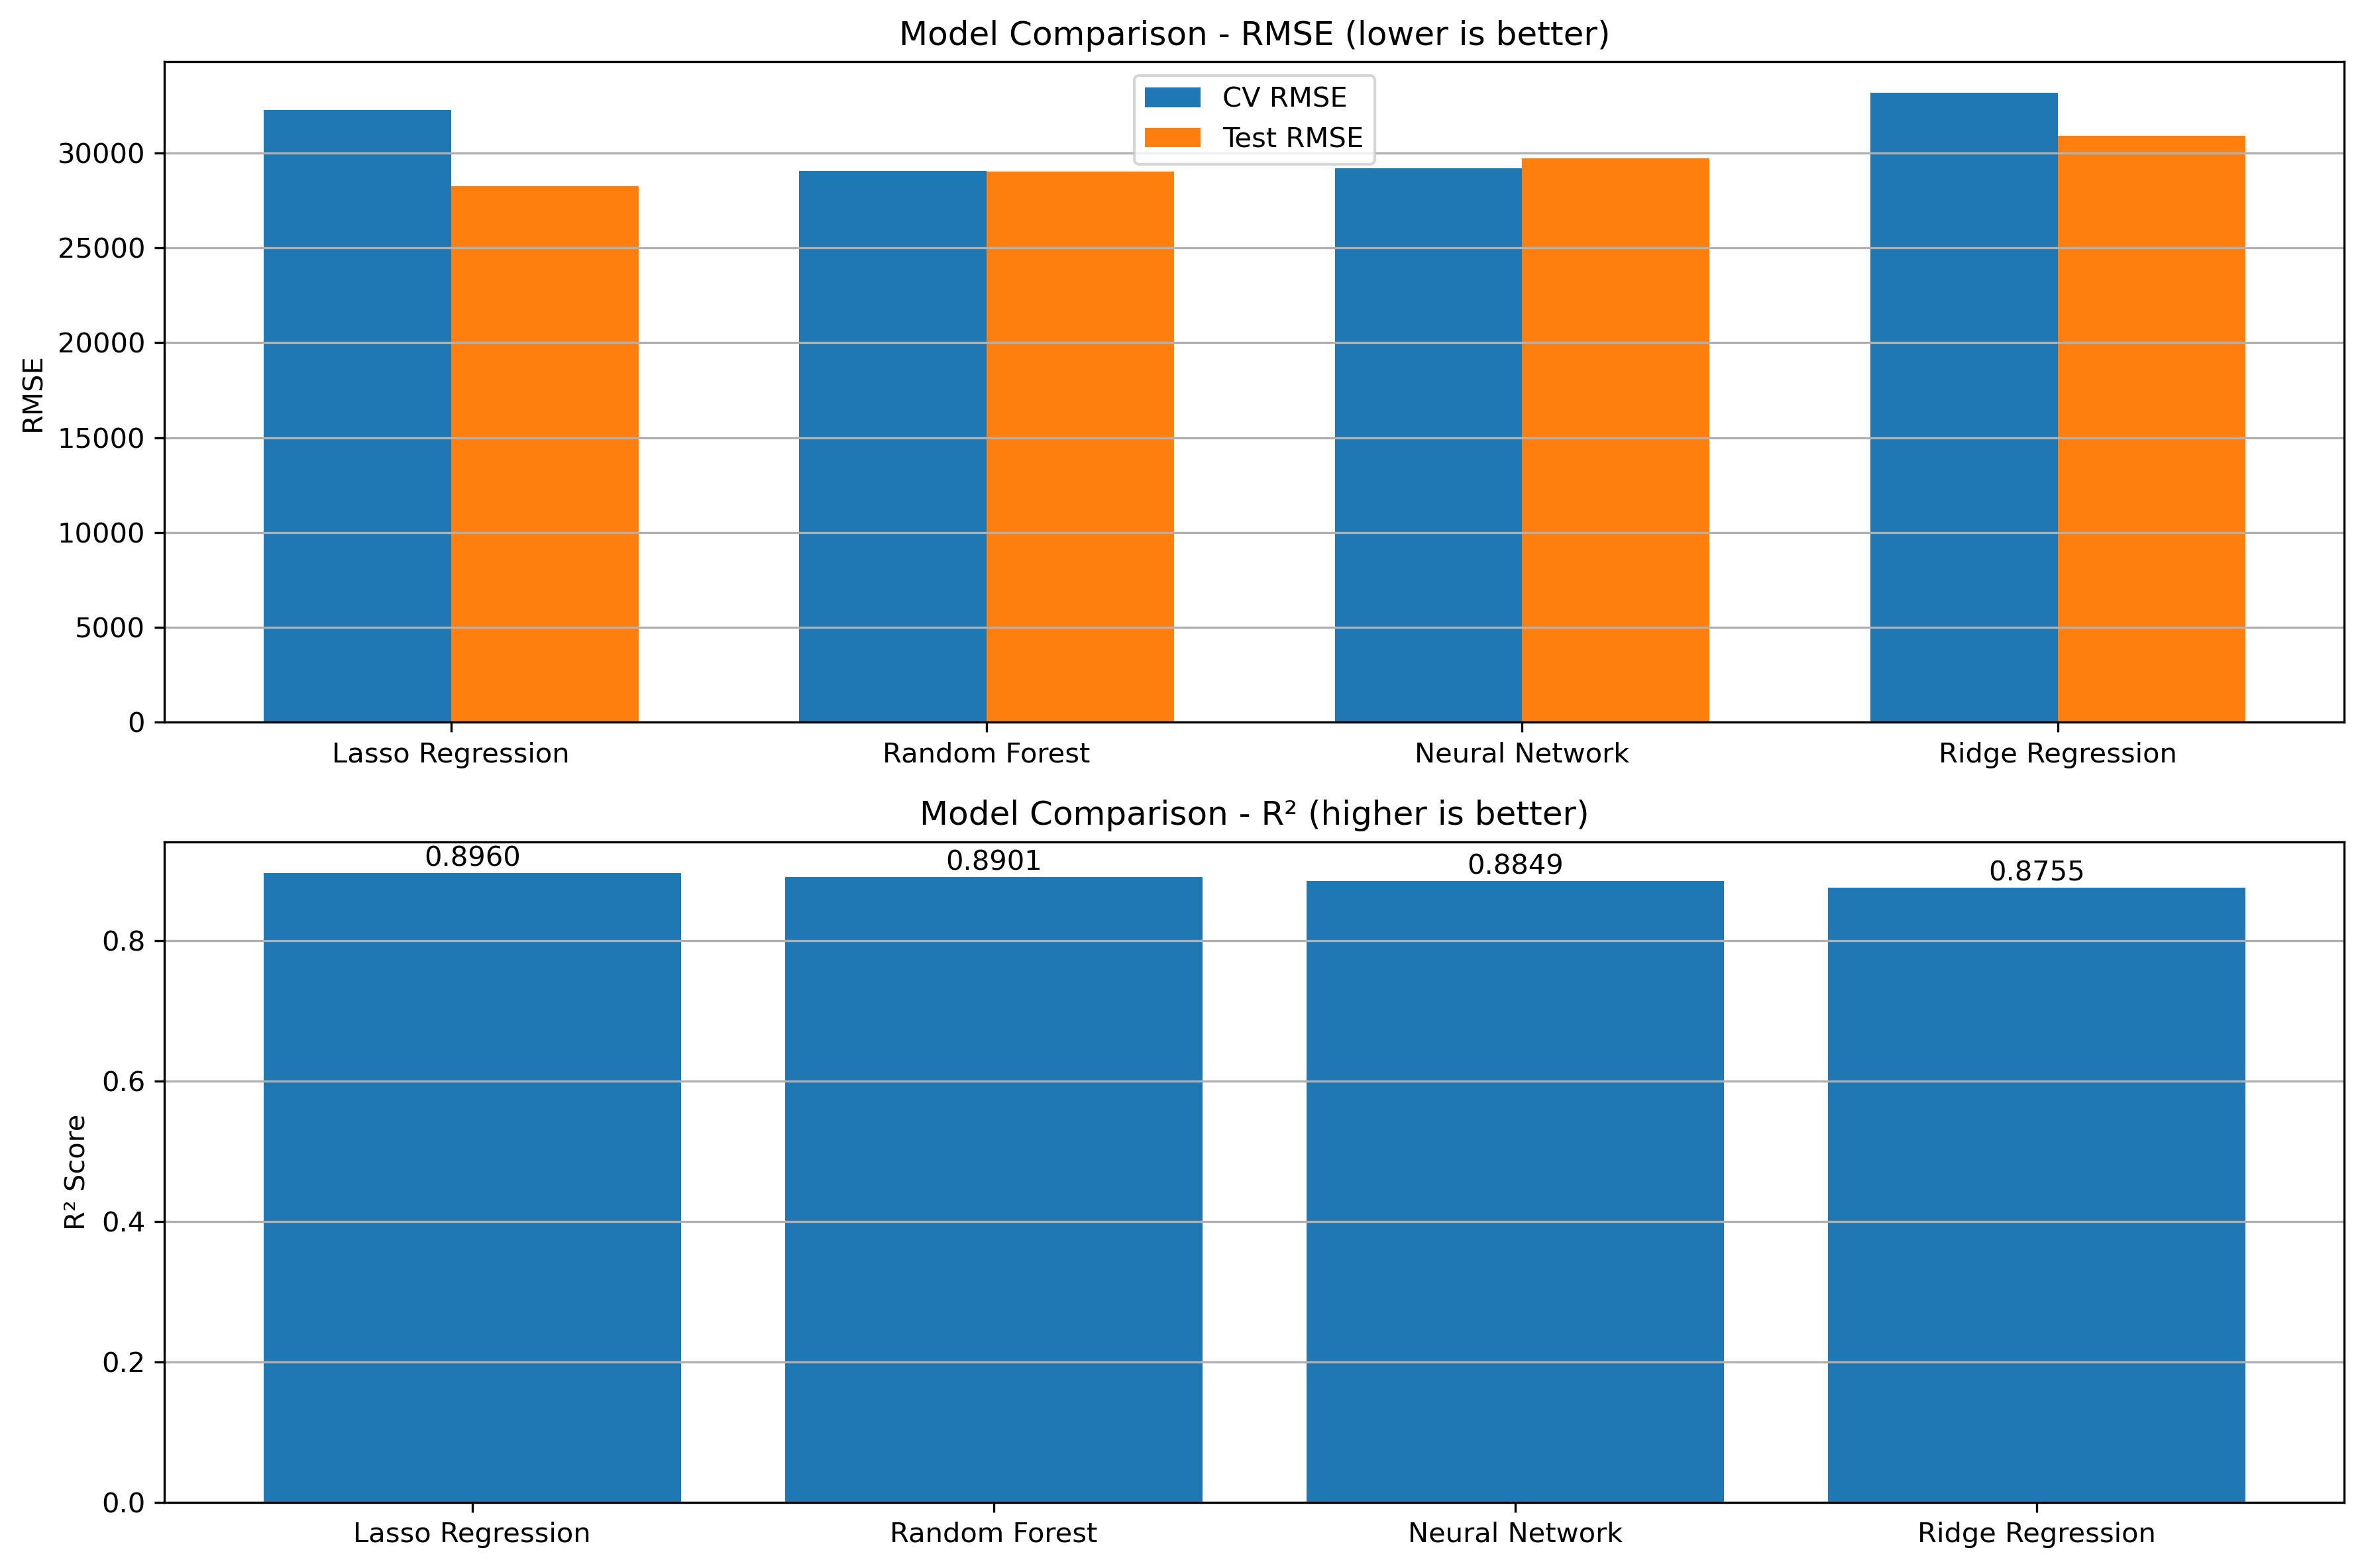
\includegraphics[width=1.0\textwidth]{figures/model_comparison.png}
    \caption{Performance Comparison Across All Four Models}
    \label{fig:model_comparison}
\end{figure}

Comparative analysis reveals several important insights:
\begin{itemize}
    \item \textbf{Lasso Regression} achieved the best overall performance with the lowest test RMSE (28,241.51) and highest R² (0.8960)
    \item \textbf{Random Forest} followed closely with test RMSE of 29,032.17 and R² of 0.8901
    \item \textbf{Neural Network} performed competitively after optimization with test RMSE of 29,713.48 and R² of 0.8849
    \item \textbf{Ridge Regression} performed well but slightly behind the other methods (RMSE: 30,907.81, R²: 0.8755)
\end{itemize}

These results highlight several key considerations for housing price prediction:
\begin{itemize}
    \item Linear models with proper regularization can perform remarkably well on this dataset
    \item Lasso's automatic feature selection provides an edge by creating a more parsimonious model
    \item Random Forest's ability to capture non-linear relationships makes it competitive
    \item Neural networks can achieve comparable performance with proper architecture and training strategies
    \item Cross-validation provides reliable estimates of generalization performance
\end{itemize}

Performance differences between all four models were relatively small, suggesting that any of these approaches could be viable in practice, with the choice depending on specific requirements for interpretability, feature selection, and implementation complexity.
\chapter{Discussion and Conclusion}
\section{Key Findings and Recommendations}
Based on the comprehensive modeling analysis with four different approaches:
\begin{itemize}
    \item Ridge Regression:
    \begin{itemize}
        \item Best for handling multicollinearity
        \item Provides stable feature importance estimates
        \item Shows which features have the strongest linear relationship with price
        \item Good performance with RMSE of 30,907.81 and R² of 0.8755
    \end{itemize}
    \item Lasso Regression:
    \begin{itemize}
        \item Offers automatic feature selection
        \item Produces sparse solutions
        \item Identifies the most crucial predictors
        \item Best overall performance with RMSE of 28,241.51 and R² of 0.8960
    \end{itemize}
    \item Random Forest:
    \begin{itemize}
        \item Captures non-linear relationships and interactions
        \item Strong predictive performance (RMSE: 29,032.17, R²: 0.8901)
        \item Less sensitive to outliers and non-normal distributions
        \item Provides reliable feature importance measurements
    \end{itemize}
    \item Neural Network:
    \begin{itemize}
        \item Achieves competitive performance with proper architecture and training (RMSE: 29,713.48, R²: 0.8849)
        \item Benefits significantly from target normalization and batch normalization
        \item Shows potential for handling complex patterns in the data
        \item Requires more careful optimization than traditional methods
    \end{itemize}
\end{itemize}

For practical implementation in real estate valuation applications, we recommend:
\begin{itemize}
    \item Use Lasso Regression when interpretability and model simplicity are important
    \item Consider Random Forest when capturing complex feature interactions is critical
    \item Employ Ridge Regression when dealing with highly correlated features
    \item Consider Neural Networks when willing to invest in optimization for competitive performance
    \item Consider ensemble approaches combining the strengths of multiple models
\end{itemize}

\section{Future Improvements}
Potential enhancements for model performance:
\begin{itemize}
    \item Ensemble methods combining multiple models, particularly Lasso, Random Forest, and Neural Network
    \item More sophisticated feature engineering based on domain knowledge
    \item Hyperparameter optimization through grid search or Bayesian optimization
    \item Integration of temporal market trends
    \item Neighborhood-specific sub-models
    \item For neural networks: 
    \begin{itemize}
        \item More complex architectures such as residual connections
        \item Advanced regularization techniques like L1 weight regularization
        \item Feature interaction layers to capture multiplicative effects
        \item Bayesian neural networks for uncertainty quantification
    \end{itemize}
\end{itemize}

\end{document} 